\documentclass[a4paper]{article}
\usepackage{a4wide,amssymb,epsfig,latexsym,multicol,multirow,array,hhline,fancyhdr}
\usepackage[utf8]{vntex, inputenc}
\usepackage[english]{babel}
\usepackage[table,xcdraw]{xcolor}
\usepackage[backend=biber,style=alphabetic,sorting=ynt]{biblatex}
\usepackage[framemethod=tikz]{mdframed}
\usepackage{amsmath}
\usepackage{lastpage}
\usepackage[lined,boxed,commentsnumbered]{algorithm2e}
\usepackage{enumerate}
\usepackage{color}
\usepackage{graphicx}							% Standard graphics package
\usepackage{tabularx, caption}
\usepackage{rotating}
\usepackage{graphics}
\usepackage{geometry}
\usepackage{setspace}
\usepackage{epsfig}
\usepackage{tikz}
\usepackage{hyperref}
\usepackage{indentfirst}
\usepackage{minted} % needs --shell-escape flag
\usepackage{gensymb}
\usepackage{float}
%\usepackage{pstcol} 								% PSTricks with the standard color package

\usepackage[english]{babel}
\usepackage[backend=biber,style=alphabetic,sorting=ynt]{biblatex}
\usepackage{csquotes}

\allowdisplaybreaks
\usetikzlibrary{arrows,snakes,backgrounds}
\hypersetup{urlcolor=blue,linkcolor=black,citecolor=red,colorlinks=true}
\addbibresource{ref.bib}
\usemintedstyle{emacs}
\numberwithin{equation}{section}
\renewcommand{\arraystretch}{1.2}

% Global style setup
\makeatletter %change font size for not having underfull hbox
\renewcommand\Huge{\@setfontsize\Huge{22pt}{18}}
\makeatother

\AtBeginDocument{\renewcommand*\contentsname{Contents}}
\AtBeginDocument{\renewcommand*\refname{References}}
%\usepackage{fancyhdr}
\setlength{\headheight}{40pt}
\pagestyle{fancy}
\fancyhead{} % clear all header fields
\fancyhead[L]{
  \begin{tabular}{rl}
    \begin{picture}(25,15)(0,0)
    \put(0,-8){
\includegraphics[width=8mm, height=8mm]{hcmut.png}}
    %\put(0,-8){\epsfig{width=10mm,figure=hcmut.eps}}
    \end{picture}
	%
\includegraphics[width=8mm, height=8mm]{hcmut.png} & %
    \begin{tabular}{l}
      \textbf{\bf \ttfamily University of Technology, Ho Chi Minh City}\\
      \textbf{\bf \ttfamily Faculty of Computer Science and Engineering}
    \end{tabular}
  \end{tabular}
}
\fancyhead[R]{
	\begin{tabular}{l}
		\tiny \bf \\
		\tiny \bf 
	\end{tabular}  }
\fancyfoot{} % clear all footer fields
\fancyfoot[L]{\scriptsize \ttfamily Assignment for Mathematical Modelling - Academic year 2020 - 2021}
\fancyfoot[R]{\scriptsize \ttfamily Page {\thepage}/\pageref{LastPage}}
\renewcommand{\headrulewidth}{0.3pt}
\renewcommand{\footrulewidth}{0.3pt}


%%%
\setcounter{secnumdepth}{4}
\setcounter{tocdepth}{3}
\makeatletter
\newcounter {subsubsubsection}[subsubsection]
\renewcommand\thesubsubsubsection{\thesubsubsection .\@alph\c@subsubsubsection}
\newcommand\subsubsubsection{\@startsection{subsubsubsection}{4}{\z@}%
                                     {-3.25ex\@plus -1ex \@minus -.2ex}%
                                     {1.5ex \@plus .2ex}%
                                     {\normalfont\normalsize\bfseries}}
\newcommand*\l@subsubsubsection{\@dottedtocline{3}{10.0em}{4.1em}}
\newcommand*{\subsubsubsectionmark}[1]{}
\makeatother


\begin{document}

\nocite{*} % Include all in bibliography

\begin{titlepage}
\begin{center}
VIETNAM NATIONAL UNIVERSITY, HO CHI MINH CITY \\
UNIVERSITY OF TECHNOLOGY \\
FACULTY OF COMPUTER SCIENCE AND ENGINEERING
\end{center}

\vspace{1cm}

\begin{figure}[h!]
\begin{center}

\includegraphics[width=3cm]{hcmut.png}
\end{center}
\end{figure}

\vspace{1cm}


\begin{center}
\begin{tabular}{c}
\multicolumn{1}{l}{\textbf{{\Large MATHEMATICAL MODELLING (CO2011)}}}\\
~~\\
\hline
\\
\multicolumn{1}{l}{\textbf{{\Large Assignment (Semester 201)}}}\\
\\
\textbf{{\Huge Dynamical systems in forecasting}}\\
\\
\textbf{{\Huge  Greenhouse Micro-climate}}\\
\\
\hline
\end{tabular}
\end{center}

\vspace{3cm}

\begin{table}[h]
\begin{tabular}{rrl}
\hspace{5 cm} Advisor: & Nguyễn Tiến Thịnh\\


\end{tabular}
\end{table}

\begin{center}
{\footnotesize HO CHI MINH CITY, JANUARY 2021}
\end{center}
\end{titlepage}


%\thispagestyle{empty}

\newpage
\tableofcontents
\newpage


%%%%%%%%%%%%%%%%%%%%%%%%%%%%%%%%%
\section*{Member list \& Workload}


\begin{center}
  \begin{tabular}{|c|c|c|l|c|}
    \hline
    \textbf{No.}       & \textbf{Fullname}                      & \textbf{Student ID}      & \textbf{Problems}              & \textbf{Percentage of work} \\
    \hline
    %%%%%Student 1%%%%%%%%%%
    \multirow{4}{*}{1} & \multirow{4}{*}{Nguyễn Đình Bảo Phúc} & \multirow{4}{*}{1852068} & \textendash{} Exercise 1    & \multirow{4}{*}{110\%}      \\
                       &                                        &                          & \textendash{} Exercise 2    &                             \\
                       &                                        &                          & \textendash{} Exercise 3    &                             \\
                       &                                        &                          & \textendash{} Exercise 4       &                             \\
                       &                                        &                          & \textendash{} Exercise 5    &                             \\
    \hline
    %%%%%Student 2%%%%%%%%%%%
    \multirow{4}{*}{2} & \multirow{4}{*}{Võ Nhật Thanh}            & \multirow{4}{*}{1852738} & \textendash{} Exercise 1    & \multirow{4}{*}{110\%}      \\
                       &                                        &                          & \textendash{} Exercise 2 &                             \\
                       &                                        &                          & \textendash{} Exercise 3    &                             \\
                       &                                        &                          & \textendash{} Exercise 4          &                             \\
                       &                                        &                          & \textendash{} Exercise 5    &                             \\
    \hline
    %%%%%Student 3%%%%%%%%%%%
    \multirow{4}{*}{3} & \multirow{4}{*}{Trần Anh Dũng}      & \multirow{4}{*}{1852306} & \textendash{} Exercise 1    & \multirow{4}{*}{110\%}      \\
                       &                                        &                          & \textendash{} Exercise 2          &                             \\
                       &                                        &                          & \textendash{} Exercise 3       &                             \\
                       &                                        &                          & \textendash{} Exercise 4          &                             \\
                       &                                        &                          & \textendash{} Exercise 5    &                             \\
    \hline
    %%%%%Student 4%%%%%%%%%%%
    \multirow{4}{*}{4} & \multirow{4}{*}{Nguyễn Minh Anh}     & \multirow{4}{*}{1852008} & \textendash{} Exercise 1    & \multirow{4}{*}{110\%}      \\
                       &                                        &                          & \textendash{} Exercise 2    &                             \\
                       &                                        &                          & \textendash{} Exercise 3          &                             \\
                       &                                        &                          & \textendash{} Exercise 4         &                             \\
                       &                                        &                          & \textendash{} Exercise 5    &                             \\
    \hline
    %%%%%Student 5%%%%%%%%%%%
    \multirow{4}{*}{5} & \multirow{4}{*}{Lê Công Trường Thọ}          & \multirow{4}{*}{1852768} & \textendash{} Exercise 2    & \multirow{4}{*}{60\%}      \\
                       &                                        &                          & \textendash{} Pending          &                             \\
                       &                                        &                          & \textendash{} Pending       &                             \\
                       &                                        &                          & \textendash{} Pending          &                             \\
    \hline
  \end{tabular}
\end{center}

\newpage
%%%%%%%%%%%%%%%%%%%%%%%%%%%%%%%%%
\section{Background}
\subsection{Introduction to dynamical systems}
Dynamical system is a system that determine how one state of the system moves to another state of the set of fixed rules over time. This system can determine the present state in terms of past states. Besides that, it can predict the future laid on the basis for the analysis of nonlinear differential.

For instance, this system can store statistic and predict the evolution of population of bacteria.

The dynamical system has two parts: \emph {The state space}, which is the set of all possible values of the state vector. \emph{The state vector} consists of a set of variables whose values can be within certain interval.

This system is classified as continuous or discrete model. The biggest difference between two kinds of this system is about the state variable, which is changed only at countable number of points in time in discrete model while being changed in a continuous way in continuous system.

For the analysis, the system is considered as linear if the system behavior satisfies some basic properties or nonlinear system which does not satisfy previous properties. If the system does not depend on the independent variable, this is the autonomous one. We should consider the time variable, if the independent variable is time, we call it time-invariant system.


Another important characteristic of a dynamical system is whether it is time dependent or not.
For time-dependent systems, the function that specifies \(\dot{x}\) or \(\Delta{x_n}\) depends on the time itself, whereas in time-independent systems, this function does not change.

\textbf{\emph{First order differential equation}} is the simplest dynamical model which has two phases: the initial state and function demonstrate the next state.
\begin{equation*}
  \begin{cases}
    $$\dot{y}(t)  &  = ay(x)$$ \\
    $$y(0)          & = y_0$$
  \end{cases}
\end{equation*}
$$a \in \mathbb{R}, \dot{y} = \frac{dy}{dx}$$\\
$$x_0 \in \mathbb{R}$$

In this assignment, we use the dynamical system especially the first order differential equation to predict the changes of $CO_2$ inside a greenhouse model (We consider the model of greenhouse in Texas, USA.) 

\subsection{Necessary and sufficient conditions for this dynamical system}
The first order differential equations in the dynamical system with the initial value $y_0$ can be re-written as: 
\begin{equation*}
  \begin{cases}
    \frac{dy}{dx} & = f(x,y) \\
    y(x_0)        & = y_0
  \end{cases}
\end{equation*}
Suppose that we have a linear differential equation $y'(x) + p(x)y = g(x)$ with the initial value $y(x_0) = y_0$. In which, p and g are continuous functions on the open interval $I = (\alpha,\beta)$, and let $t_0 \in (\alpha,\beta)$. Then for each $t \in I$ there exists a unique solution $y = \phi (t)$ to the differential equation $\frac{dy}{dx} + p(x)y = g(x)$ that also satisfies the initial value condition that $y(x_0) = y_0$.

\subsection{Examples of solvable first-order differential equations and their exact solutions}
\textbf{- First equation:}
\begin{equation*}
  \begin{cases}
    \frac{dy}{dt} & = y - t^2 +1 \\
    y(0)          & = 0.5
  \end{cases}
\end{equation*}

This can be put into a form of a first-order linear differential equation: \(\frac{dy}{dx} +P(x)y  = Q(x)\)\\
where P and Q are continuous functions on a given interval.\\

And general solution: ~~ \( y = e^{-\int P(x)dx}(\int e^{\int P(x)dx}.Q(x) dx +C) \)\\

We have, ~~ $\frac{dy}{dt} = y-t^2+1$ ~~ $ \Rightarrow \frac{dy}{dt} -y = -t^2+1 $ in which \( P(t)=-1~ and~ Q(t)=-t^2+1 \)

\begin{align*}
  \Rightarrow ~~ y &= e^{-\int P(t)dt}(\int e^{\int P(t)dt}\cdot Q(t) t +C )\\
  y &= e^{-\int -1dt}(\int e^{\int 1dt}\cdot(-t^2+1)dt +C)\\
  y &= e^-t(\int e^t\cdot(-t^2+1)dt +C)\\
  y &= e^-t(e^t\cdot(t+1)^2 +C)\\
  y &= (t+1)^2 +e^t\cdot C\\
\end{align*}
Combining the general solution with the given initial value, we obtain
\begin{align*}
  0.5 & = y(0) = (0+1)^2 +e^0\cdot C =1+C \\
  C & = -0.5
\end{align*}
Thus, the particular solution is
\begin{align*}
   y = (t+1)^2 -0.5e^t\\
\end{align*} 

\textbf{- Second equation:}
\begin{equation*}
  \begin{cases}
    \frac{dy}{dt} & = -1.2y + 7e^{-0.3t}  \\
    y(0)          & = 3
  \end{cases}
\end{equation*}

This can be put into a form of a first-order linear differential equation: \(\frac{dy}{dx} +P(x)y  = Q(x)\)\\
where P and Q are continuous functions on a given interval.\\

And general solution: \( y = e^{-\int P(x)dx}(\int e^{\int P(x)dx}.Q(x) dx +C) \)\\

We have, $\frac{dy}{dt} = -1.2y + 7e^{-0.3t}$ ~~ $ \Rightarrow \frac{dy}{dt} +1.2y = 7e^{-0.3t}$ in which \( P(t)=1.2~~and~~Q(t)=7e^{-0.3t} \)

\begin{align*}
  \Rightarrow ~~ y &= e^{-\int P(t)dt}(\int e^{\int P(t)dt}\cdot Q(t) t +C )\\
  y &= e^{-\int 1.2dt}(\int e^{\int 1.2dt}\cdot7e^{-0.3t}dt +C)\\
  y &= 7e^{-1.2t}(\int e^{1.2t}\cdot e^{-0.3t}dt +C)\\
  y &= 7e^{-1.2t}(\int e^{0.9t}dt +C)\\
  y &= 7e^{-1.2t}(\frac{e^{0.9t}}{0.9} +C)\\
  y &= \frac{70}{9}e^{-0.3t}+7e^{-1.2t}\cdot C\\
\end{align*}

Combining the general solution with the given initial value, we obtain
\begin{align*}
  3 & = y(0) = \frac{70}{9}e^{-0.3\cdot 0}+7e^{-1.2\cdot 0}\cdot C =\frac{70}{9}+7C \\
  7C & = \frac{-43}{9}
\end{align*}

Thus, the particular solution is
\begin{align*}
   y = \frac{70}{9}e^{-0.3t}-\frac{43}{9}e^{-1.2t}\\
\end{align*}



\subsection{Explicit Euler and Explicit Runge–Kutta of order 4 algorithms}
\subsubsection{Explicit Euler algorithm} \label{sssec:explicit_euler}
Given an initial value problem
\begin{equation*}
  \begin{cases}
    \frac{dy}{dt} = f(t,y) \\
    y(t_0) = y_0
  \end{cases}
\end{equation*}


The operation which can not be evaluated numerically obviously is the limit h → 0, that defines the derivative
\begin{align*}
  \frac{dy}{dt} = \lim_{h \rightarrow 0} \frac{y(t + h) - y(t)}{h}
\end{align*}

However, for any positive (small) h, the finite difference \(\frac{y(t + h) - y(t)}{h}\) can easily be evaluated. Thus,we can have the following approximation:
\begin{align*}
  \frac{dy}{dt} \approx \frac{y(t + h) - y(t)}{h}
\end{align*}
By definition, it is an approximation of the derivative
y'(t). Let us therefore approximate the differential equation \(\frac{dy}{dt} = f(t,y)\) by the difference equation

\begin{align*}
  f(t,y(t)) \approx  \frac{y(t + h) - y(t)}{h} 
\end{align*}

Given y at time t, one can compute y at the later time t + h, by solving the difference equation
\begin{align*}
  y(t + h) \approx y(t) + h \cdot f(t,y(t))
\end{align*}

This is exactly one step of the explicit Euler method. Introducing the notation \( t_{n+1} = t_n + h \). Exact value of solution at \(t_k\) is denoted by \(y(t_k)\), approximate value is denoted by \(y_k\). We have Euler’s formula
\begin{align*}
  y(t_{n+1}) \approx y_{n+1} = y_n + h \cdot f(t_n, y_n)
\end{align*}

We can calculate \(y(t_k)\) at any time \(t_k\) since we are provided with the initial condition \(y(t_0) = y_0\)
That is the approximation steps of the Explicit Euler algorithm to solve general first-order differential equations.


\subsubsection{Explicit Runge–Kutta of order 4 algorithm}
The formula for the fourth order Runge-Kutta method (RK4) is given below. Consider the problem
\begin{equation*}
  \begin{cases}
    \frac{dy}{dt} = f(t,y) \\
    y(t_0) = y_0
  \end{cases}
\end{equation*}

Define h to be the time step size and \(t_n = t_0 + n\cdot h\). Exact value of solution at \(t_n\) is denoted by \(y(t_n)\), approximate value is denoted by \(y_n\). Then the following formula

\begin{align*}
  k_1 & = h\cdot f(t_n, y_n)                                \\
  k_2 & = h\cdot f(t_n + \frac{h}{2}, y_n + \frac{k_1}{2}) \\
  k_3 & = h\cdot f(t_n + \frac{h}{2}, y_n + \frac{k_2}{2}) \\
  k_4 & = h\cdot f(t_n + h, y_n + k_3)\\
    y_{n+1} &= y_n + \frac{1}{6}(k_1 + 2k_2 + 2k_3 + k_4) \\
\end{align*}

computes an approximate solution, that is \(y_n \approx y(t_n)\).\\

This method has local truncation error \(O(h^4)\), provided the
solution y(t) has five continuous derivatives. We introduce the notation k1, k2, k3, k4 into
the method is to eliminate the need for successive nesting in the second variable of  \(f(t,y)\).

	
\subsection{Applying Euler and Runge-Kutta algorithms, give approximate solution of the above examples}
We use \(h = 0.2\) for the first system of equations and  \(h = 0.5\) for second system of equations.
\subsubsection{Explicit Euler}
\textbf{First system of equations:}
\begin{equation*}
  \begin{cases}
    \frac{dy}{dt} & = y - t^2 +1 \\
    y(0)          & = 0.5
  \end{cases}
\end{equation*}

And its exact solution:
\begin{align*}
   y = (t+1)^2 -0.5e^t
\end{align*} 

With \(t_0 = 0, h=0.2 ~~\rightarrow ~~ y_0 = 0.5\) and \(t_k = t_0 + k \cdot h = 0.2k\).\\

Applying the explicit Euler's formula for approximate solution as stated in~\ref{sssec:explicit_euler}, we have:

\begin{align*}
  y_1 & = y_0 + h\cdot(y_0-t_0^2+1)                                     \\
      & = 0.5 + 0.2 \cdot(0.5-0^2+1) =0.8                                                                       \\
 y_2 & = y_1 + h\cdot(y_1-t_1^2+1)                                     \\
      & = 0.8 + 0.2 \cdot(0.8-0.2^2+1) =1.152                                          \\
   y_3 & = y_2 + h\cdot(y_2-t_2^2+1)                                     \\
      & = 1.152 + 0.2 \cdot(1.152-0.4^2+1) =1.5504  
\\
 y_4 & = y_3 + h\cdot(y_3-t_3^2+1)                                     \\
      & = 1.5504 + 0.2 \cdot(1.5504-0.6^2+1) =1.98848   
      \\
       y_5 & = y_4 + h\cdot(y_4-t_4^2+1)                                     \\
      & = 1.98848 + 0.2 \cdot(1.98848-0.8^2+1) =2.458176  
\end{align*}

 Compare the appoximate solution ( \(y_k\) ) and exact solution  ( \(y(t_k)\) ) we have the  table for explicit Euler method as follows:
 
 \begin{table}[H]
 \centering
\begin{tabular}{|l|l|l|l|l|}
\hline
k & \(t_k\)  &  Approx.solution \(y_k\)       &  Exact solution \(y(t_k)\)     & \(|y(t_k)-y_k|\) \\ \hline
0 & 0.0 & 0.5000000 & 0.5000000 & 0.0000000   \\ \hline
1 & 0.2 & 0.8000000 & 0.8292986 & 0.0292986   \\ \hline
2 & 0.4 & 1.1520000 & 1.2140877 & 0.0620877   \\ \hline
3 & 0.6 & 1.5504000 & 1.6489406 & 0.0985406   \\ \hline
4 & 0.8 & 1.9884800 & 2.1272295 & 0.1387495   \\ \hline
5 & 1.0 & 2.4581760 & 2.6408591 & 0.1826831   \\ \hline
\end{tabular}
\end{table}
 
\textbf{Second system of equations:}
\begin{equation*}
  \begin{cases}
    \frac{dy}{dt} & = -1.2y + 7e^{-0.3t}  \\
    y(0)          & = 3
  \end{cases}
\end{equation*}

And its exact solution:
\begin{align*}
   y = \frac{70}{9}e^{-0.3t}-\frac{43}{9}e^{-1.2t}\\
\end{align*}

With \(t_0 = 0, h=0.5 ~~\rightarrow ~~ y_0 = 3\) and \(t_k = t_0 + k \cdot h = 0.5k\).\\

Applying the explicit Euler's formula for approximate solution as stated in~\ref{sssec:explicit_euler}, we have: 

\begin{align*}
  y_1 & = y_0 + h\cdot(-1.2\cdot y_0 + 7e^{-0.3\cdot t_0})                                     \\
      & = 3 + 0.5 \cdot(-1.2\cdot 3 + 7e^{-0.3\cdot 0}) =4.7                                                         \\
 y_2 & = y_1 + h\cdot(-1.2\cdot y_1 + 7e^{-0.3\cdot t_1})                                     \\
      & = 4.7 + 0.5 \cdot(-1.2\cdot 4.7 + 7e^{-0.3\cdot 0.5}) =4.892477917                                          \\
   y_3 & = y_2 + h\cdot(-1.2\cdot y_2 + 7e^{-0.3\cdot t_2})                                     \\
      & = 4.892477917  + 0.5 \cdot(-1.2\cdot 4.892477917  + 7e^{-0.3\cdot 1}) =4.549854939  
\\
 y_4 & = y_3 + h\cdot(-1.2\cdot y_3 + 7e^{-0.3\cdot t_3})                                     \\
      & = 4.549854939  + 0.5 \cdot(-1.2\cdot 4.549854939  + 7e^{-0.3\cdot 1.5}) =4.051640506 
      \\
       y_5 & = y_4 + h\cdot(-1.2\cdot y_4 + 7e^{-0.3\cdot t_4})                                     \\
     & = 4.051640506  + 0.5 \cdot(-1.2\cdot 4.051640506  + 7e^{-0.3\cdot 2}) =3.541496929  
\end{align*}

 Compare the appoximate solution ( \(y_k\) ) and exact solution  ( \(y(t_k)\) ) we have the  table for explicit Euler method as follows:
 
  \begin{table}[H]
 \centering
\begin{tabular}{|l|l|l|l|l|}
\hline
k & \(t_k\)  &  Approx.solution \(y_k\)       &  Exact solution \(y(t_k)\)     & \(|y(t_k)-y_k|\) \\ \hline
0 & 0.0 & 3.000 & 3.0000 & 0.0000   \\ \hline
1 & 0.5 & 4.700 & 4.0720 & 0.6277   \\ \hline
2 & 1.0 & 4.893 & 4.4323 & 0.5696   \\ \hline
3 & 1.5 & 4.550 & 4.1700 & 0.3803   \\ \hline
4 & 2.0 & 4.052 & 3.8350 & 0.2165   \\ \hline
5 & 2.5 & 3.542 & 3.4360 & 0.1054   \\ \hline
\end{tabular}
\end{table}
 
 
 
\subsubsection{Explicit RK4}
\textbf{First system of equations:}
\begin{equation*}
  \begin{cases}
    \frac{dy}{dt} & = y - t^2 +1 \\
    y(0)          & = 0.5
  \end{cases}
\end{equation*}

And its exact solution:
\begin{align*}
   y = (t+1)^2 -0.5e^t
\end{align*} 

With \(t_0 = 0, h=0.2 ~~\rightarrow ~~ y_0 = 0.5\) and \(t_k = t_0 + k \cdot h = 0.2k\).\\

From t = 0 to t = 1 with step size h = 0.2, it takes 5 steps: \(t_0 = 0\), \(t1 = 0.2\), \(t2 = 0.4\), \(t3 = 0.6\) , \(t4 = 0.8\), \(t5 = 1\).\\

\underline{\textit{Step 0:}} \(t_0=0\) , \(y_0=0.5\) \\

\underline{\textit{Step 1:}} \(t_1=0.2\)\\

  $k_1 = hf(t_0,~ y_0) = 0.2f(0, 0.5) = 0.3$\\
  
  $k_2 = hf \left(t_0 + \frac{h}{2},~ y_0 + \frac{k_1}{2}\right) = 0.2f(0.1,~ 0.5+\frac{0.3}{2}) = 0.328$\\  
  
  $k_3 = hf \left(t_0 + \frac{h}{2},~ y_0 + \frac{k_2}{2}\right) = 0.2f(0.1,~ 0.5+\frac{0.328}{2}) = 0.3308$ \\
  
  $k_4 = hf(t_0 + h,~ y_0 + k_3) = 0.2f(0.2,~ 0.5+0.3308) = 0.35816$\\
  
  $\rightarrow y_1 = y_0 + \frac{1}{6}(k_1 + 2k_2 + 2k_3 + k_4)$\\
  
  $= 0.5 + \frac{1}{6}(0.3 + 2 * 0.328 + 2 * 0.3308 + 0.35816 )$\\ 
  
  $\approx 0.82929333333$\\

\underline{\textit{Step 2:}} \(t_2=0.4\)\\

  $k_1 = hf(t_1,~ y_1) = 0.2f(0.2,0.82929333333) = 0.3578586667$\\
  
  $k_2 = hf \left(t_1 + \frac{h}{2},~ y_1 + \frac{k_1}{2}\right) = 0.2f(0.3,~ 0.82929333333 + \frac{0.3578586667}{2}) = 0.3836445333$\\
  
  $k_3 = hf \left(t_1 + \frac{h}{2},~ y_1 + \frac{k_2}{2}\right) = 0.2f(0.3,~ 0.82929333333 + \frac{0.3836445333}{2}) = 0.338622312$\\
  
  $k_4 = hf(t_1 + h,~ y_1 + k_3) = 0.2f(0.4,~ 0.82929333333 + 0.338622312) = 0.4111032907$\\
  
  $\rightarrow y_2 = y_1 + \frac{1}{6}(k_1 + 2k_2 + 2k_3 + k_4)$\\
  
  $= 0.82929333333 + \frac{1}{6} \left(0.3578586667 + 2*0.3836445333 + 2*0.338622312 + 0.4111032907\right)$\\   
  
  $\approx 1.214076211$\\

\underline{\textit{Step 3:}} \(t_3=0.6\)\\

    $k_1 = hf(t_2,~ y_2) = 0.2f(0.4,1.214076211) = 0.4108152421$\\
  
    $k_2 = hf\left(t_2 + \frac{h}{2},~ y_2 + \frac{k_1}{2}\right) = 0.2f(0.5,~ 1.214076211 + \frac{0.4108152421}{2}) = 0.4338967663$\\
    
    $k_3 =hf\left(t_2 + \frac{h}{2},~ y_2 + \frac{k_2}{2}\right) = 0.2f(0.5,~ 1.214076211 + \frac{0.4338967663}{2}) = 0.4362049188$\\
    
    $k_4 = hf(t_2 + h,~ y_2 + k_3) = 0.2f(0.6,~ 1.214076211 + 0.4362049188) = 0.4580562259$\\
    
    $\rightarrow y_3 = y_2 + \frac{1}{6}(k_1 + 2k_2 + 2k_3 + k_4)$\\ 
    
    $= 1.214076211 + \frac{1}{6} \left(0.4108152421 + 2*0.4338967663 + 2*  0.4362049188 + 0.4580562259\right)$\\
    
    $\approx 1.648922017$\\

\underline{\textit{Step 4:}} \(t_4=0.8\)\\

  $k_1 = hf(t_3,~ y_3) = 0.2f(0.6,1.648922017) = 0.4577844034$\\
  
  $k_2 = hf\left(t_3 + \frac{h}{2},~ y_3 + \frac{k_1}{2}\right) = 0.2f(0.7,~ 1.648922017 + \frac{0.4577844034}{2}) = 0.4775628437$\\
  
  $k_3 = hf\left(t_3 + \frac{h}{2},~ y_3 + \frac{k_2}{2}\right) = 0.2f(0.7,~ 1.648922017 + \frac{0.4775628437}{2}) = 0.4795406878$\\
  
  $k_4 = hf(t_3 + h,~ y_3 + k_3) = 0.2f(0.8,~ 1.648922017+0.4795406878) = 0.497692541$\\
  
  $\rightarrow y_4 = y_3 + \frac{1}{6}(k_1 + 2k_2 + 2k_3 + k_4)$\\ 
  
  $= 1.648922017 + \frac{1}{6} \left(0.4577844034 + 2*0.4775628437 + 2*0.4795406878 + 0.497692541\right)$\\  
  
  $\approx 2.127202685$\\

\underline{\textit{Step 5:}} \(t_5=1\)\\

  $k_1 = hf(t_4,~ y_4) = 0.2f(0.8,2.127202685 = 0.497440537$\\
  
  $k_2 = hf\left(t_4 + \frac{h}{2},~ y_4 + \frac{k_1}{2}\right) = 0.2f(0.9,~ 2.127202685 + \frac{0.497440537}{2}) = 0.5131845907$\\
  
  $k_3 = hf\left(t_4 + \frac{h}{2},~ y_4 + \frac{k_2}{2}\right) = 0.2f(0.9,~ 2.127202685 + \frac{0.5131845907}{2}) = 0.5147589961$\\
  
  $k_4 = hf(t_4 + h,~ y_4 + k_3) = 0.2f(1,~ 2.127202685 + 0.5147589961) = 0.5283923362$\\
  
  $\rightarrow y_5 = y_4 + \frac{1}{6}(k_1 + 2k_2 + 2k_3 + k_4)$\\
  
  $= 2.127202685 + \frac{1}{6} \left(0.497440537 + 2*0.5131845907 + 2*0.5147589961 + 0.5283923362\right)$\\ 
  
  $\approx 2.640822693$\\

 Compare the appoximate solution (\(y_k\)) and exact solution (\(y(t_k)\)) we have the  table for explicit RK4 method as follows:

\begin{table}[H]
\centering
\begin{tabular}{|c|c|c|c|}
\hline
\multicolumn{1}{|c|}{\(t_k\)} & \multicolumn{1}{c|}{\begin{tabular}[c]{@{}c@{}}Exact solution \\ \(y_k\) \end{tabular}} & \multicolumn{1}{c|}{\begin{tabular}[c]{@{}c@{}} RK-4 solution\\ \(y(t_k)\) \end{tabular}} & \multicolumn{1}{c|}{\begin{tabular}[c]{@{}c@{}}Error\\ \(|y(t_k) - y_k|\) \end{tabular}}\\ \hline
0.0                      & 0.5                                                                               & 0.5                                                                                & 0                                                                                \\ \hline
0.2                      & 0.829298620919915                                                                 & 0.829293333333333                                                                  & 0.000005287586582                                                                \\ \hline
0.4                      & 1.214087651179365                                                                 & 1.214076210666667                                                                  & 0.000011440512698                                                                \\ \hline
0.6                      & 1.648940599804746                                                                 & 1.648922017041600                                                                  & 0.000018582763146                                                                \\ \hline
0.8                      & 2.127229535753766                                                                 & 2.127202684947944                                                                  & 0.000026850805823                                                                \\ \hline
1.0                      & 2.640859085770477                                                                 & 2.640822692728752                                                                  & 0.000036393041726                                                                \\ \hline
\end{tabular}
\end{table}

\textbf{Second system of equations:}
\begin{equation*}
  \begin{cases}
    \frac{dy}{dt} & = -1.2y + 7e^{-0.3t}  \\
    y(0)          & = 3
  \end{cases}
\end{equation*}

And its exact solution:
   $y = \frac{70}{9}e^{-0.3t}-\frac{43}{9}e^{-1.2t}$\\
With \(t_0 = 0, h=0.5 ~~\rightarrow ~~ y_0 = 3\) and \(t_k = t_0 + kh = 0.5k\).\\

From t = 0 to t = 2.5 with step size h = 0.5, it takes 5 steps: \(t_0 = 0\), \(t1 = 0.5\), \(t2 = 1.0\), \(t3 = 1.5\) , \(t4 = 2.0\), \(t5 = 2.5\).\\

\underline{\textit{Step 0:}} \(t_0=0\) , \(y_0=3\) \\

\underline{\textit{Step 1:}} \(t_1=0.5\)\\

  $k_1 = hf(t_0, y_0) = 0.5f(0, 3) = 1.7$\\
  
  $k_2 = hf\left(t_0 + \frac{h}{2}, y_0 + \frac{k_1}{2}\right) = 0.5f(0.25, 3 + \frac{1.7}{2}) = 0.9371022021$\\
  
  $k_3 = hf\left(t_0 + \frac{h}{2}, y_0 + \frac{k_2}{2}\right) = 0.5f(0.25, 3 + \frac{0.9371022021}{2}) = 1.165971542$\\
  
  $k_4 = hf(t_0 + h, y_0 + k_3) = 0.5f(0.5, 3+ 1.165971542) = 0.5128949926$\\
  
  $\rightarrow y_1 = y_0 + \frac{1}{6}(k_1 + 2k_2 + 2k_3 + k_4)$\\
  
  $= 3 + \frac{1}{6} (1.7 + 2*0.9371022021 + 2*0.9371022021 + 0.5128949926)$\\   
  $\approx 4.069840413$\\

\underline{\textit{Step 2:}} \(t_2=1.0\)
\begin{alignat*}{4}
  k_1 & = h\cdot f(t_1, y_1)                                            &  & = 0.5\cdot f(0.5,4.069840413)                    &  & = 0.5705736695                \\
  k_2 & = h\cdot f \left(t_1 + \frac{h}{2}, y_1 + \frac{k_1}{2}\right) &  & = 0.5\cdot f(0.75, 4.069840413+\frac{0.5705736695 }{2})                  &  & = 0.1817304168               \\
  k_3 & = h\cdot f \left(t_1 + \frac{h}{2}, y_1 + \frac{k_2}{2}\right) &  & = 0.5\cdot f(0.75, 4.069840413+\frac{0.1817304168}{2})               &  & = 0.2983833926 \\
  k_4 & = h\cdot f(t_1 + h, y_1 + k_3)                                 &  & = 0.5\cdot f(1.0, 4.069840413+0.2983833926) &  & = -0.02807051118 
\end{alignat*}
\begin{align*}
     \rightarrow y_2 & = y_1 + \frac{1}{6}(k_1 + 2k_2 + 2k_3 + k_4)                                                             \\
       &= 4.069840413 + \frac{1}{6} \left(0.5705736695 + 2 \cdot 0.1817304168  + 2 \cdot  0.2983833926 + -0.02807051118\right) \\               
      & \approx 4.320295543
\end{align*}

\underline{\textit{Step 3:}} \(t_3=1.5\)
\begin{alignat*}{4}
  k_1 & = h\cdot f(t_1, y_1)                                            &  & = 0.5\cdot f(1,4.320295543)                    &  & = 0.000686446               \\
  k_2 & = h\cdot f \left(t_1 + \frac{h}{2}, y_1 + \frac{k_1}{2}\right) &  & = 0.5\cdot f(1.25, 4.320295543+\frac{0.000686446 }{2})                  &  & = -0.1868707839               \\
  k_3 & = h\cdot f \left(t_1 + \frac{h}{2}, y_1 + \frac{k_2}{2}\right) &  & = 0.5\cdot f(1.25, 4.320295543+\frac{-0.1868707839}{2})               &  & = -0.1306036148 \\
  k_4 & = h\cdot f(t_1 + h, y_1 + k_3)                                 &  & = 0.5\cdot f(1.5, 4.320295543+-0.1306036148) &  & = -0.2821166262
\end{alignat*}
\begin{align*}
     \rightarrow y_3 & = y_2 + \frac{1}{6}(k_1 + 2k_2 + 2k_3 + k_4)                                                             \\
       &= 4.320295543 + \frac{1}{6} \left(0.000686446 + 2 \cdot -0.1868707839   + 2 \cdot  -0.1306036148 + -0.2821166262\right) \\               
      & \approx 4.167565713
\end{align*}

\underline{\textit{Step 4:}} \(t_4=2.0\)
\begin{alignat*}{4}
  k_1 & = h\cdot f(t_1, y_1)                                            &  & = 0.5\cdot f(1.5,4.167565713)                    &  & = -0.2688408973               \\
  k_2 & = h\cdot f \left(t_1 + \frac{h}{2}, y_1 + \frac{k_1}{2}\right) &  & = 0.5\cdot f(1.75, 4.167565713+\frac{-0.2688408973 }{2})                  &  & = -0.3494433835              \\
  k_3 & = h\cdot f \left(t_1 + \frac{h}{2}, y_1 + \frac{k_2}{2}\right) &  & = 0.5\cdot f(1.75, 4.167565713+\frac{-0.3494433835}{2})               &  & = -0.3252626377 \\
  k_4 & = h\cdot f(t_1 + h, y_1 + k_3)                                 &  & = 0.5\cdot f(2, 4.167565713+-0.3252626377) &  & = -0.3845411191
\end{alignat*}
\begin{align*}
     \rightarrow y_4 & = y_3 + \frac{1}{6}(k_1 + 2k_2 + 2k_3 + k_4)                                                             \\
       &= 4.167565713 + \frac{1}{6} \left(-0.2688408973 + 2 \cdot -0.3494433835    + 2 \cdot  -0.3252626377 + -0.3845411191\right) \\               
      & \approx 3.833766704
\end{align*}

\underline{\textit{Step 5:}} \(t_5=2.5\)
\begin{alignat*}{4}
  k_1 & = h\cdot f(t_1, y_1)                                            &  & = 0.5\cdot f(2.0,3.833766704)                    &  & = -0.3794192958               \\
  k_2 & = h\cdot f \left(t_1 + \frac{h}{2}, y_1 + \frac{k_1}{2}\right) &  & = 0.5\cdot f(2.25, 3.833766704+\frac{-0.3794192958   }{2})                  &  & = -0.4043867613              \\
  k_3 & = h\cdot f \left(t_1 + \frac{h}{2}, y_1 + \frac{k_2}{2}\right) &  & = 0.5\cdot f(2.25, 3.833766704+\frac{-0.4043867613}{2})               &  & = -0.3968965216 \\
  k_4 & = h\cdot f(t_1 + h, y_1 + k_3)                                 &  & = 0.5\cdot f(2.5, 3.833766704+-0.3968965216) &  & = -0.4088391746
\end{alignat*}
\begin{align*}
     \rightarrow y_5 & = y_4 + \frac{1}{6}(k_1 + 2k_2 + 2k_3 + k_4)                                                             \\
       &= 3.833766704 + \frac{1}{6} \left(-0.3794192958 + 2 \cdot -0.4043867613    + 2 \cdot  -0.3968965216 + -0.3968965216\right) \\               
      & \approx 3.435295864
\end{align*}

 Compare the appoximate solution ( \(y_k\) ) and exact solution  ( \(y(t_k)\) ) we have the  table for explicit RK4 method as follows:

\begin{table}[H]
\centering
\begin{tabular}{|l|l|l|l|}
\hline
\multicolumn{1}{|c|}{\(t_k\)} & \multicolumn{1}{c|}{\begin{tabular}[c]{@{}c@{}}Exact solution \\ \(y_k\)\end{tabular}} & \multicolumn{1}{c|}{\begin{tabular}[c]{@{}c@{}} RK-4 solution \\ \(y(t_k)\) \end{tabular}} & \multicolumn{1}{c|}{\begin{tabular}[c]{@{}c@{}}Error\\ \(|y(t_k) - y_k|\)\end{tabular}} \\ \hline
0.0                      & 3                                                                               & 3                                                                                & 0                                                                                \\ \hline
0.5                      & 4.072295333                                                                 & 4.069840413                                                                      & 0.002454920                                                                \\ \hline
1.0                      & 4.322880482                                                               & 4.320295543                                                                  & 0.002584939                                                                \\ \hline
1.5                      & 4.169568713                                                               & 4.167565713                                                                 & 0.002003000                                                                \\ \hline
2.0                      & 3.835104726                                                                 & 3.833766704                                                                  & 0.001338022                                                                \\ \hline
2.5                      & 3.436090528                                                                 & 3.435295864                                                                  & 0.000794664                                                                \\ \hline
\end{tabular}
\end{table}

\newpage
%%%%%%%%%%%%%%%%%%%%%%%%%%%%%%%%%
\section{Exercise 2}
	\subsection{Restate the model of \(CO_2\) concentration}
\subsubsection{\(CO_2\) exchange}
In nature, there are several factors that affect to the crop growth. In order to maximize the crop yield, it is necessary to control and predict these factors. The first factor we considered is \(CO_2\) concentration. A greenhouse with thermal screen, which can help us not only on controlling \(CO_2\) concentration but also light, temperature. Which means we can better control the climate to maximize the growth of crop.
\begin{figure}[H]
  \centering
  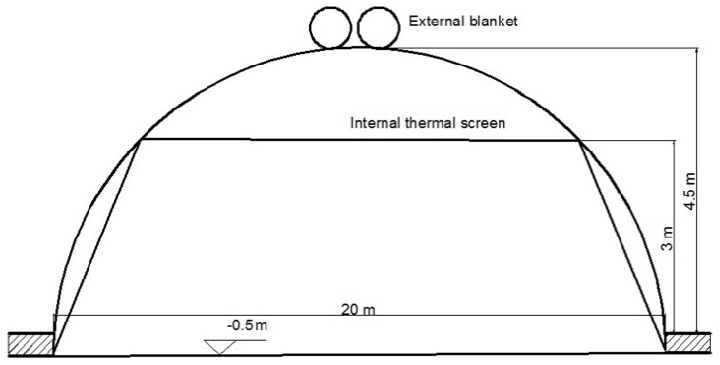
\includegraphics[width=11cm]{thrscr.png}
  \caption{Greenhouse thermal screen}\label{fig:thrscr}
\end{figure}

In figure~\ref{fig:thrscr}, As you can see the greenhouse model is divided into two compartments by internal thermal screen. One part above the screen and the below one. 
The concentrations of \(CO_2\) in two of the compartments are described as the figure below.
\begin{figure}[H]
  \centering
  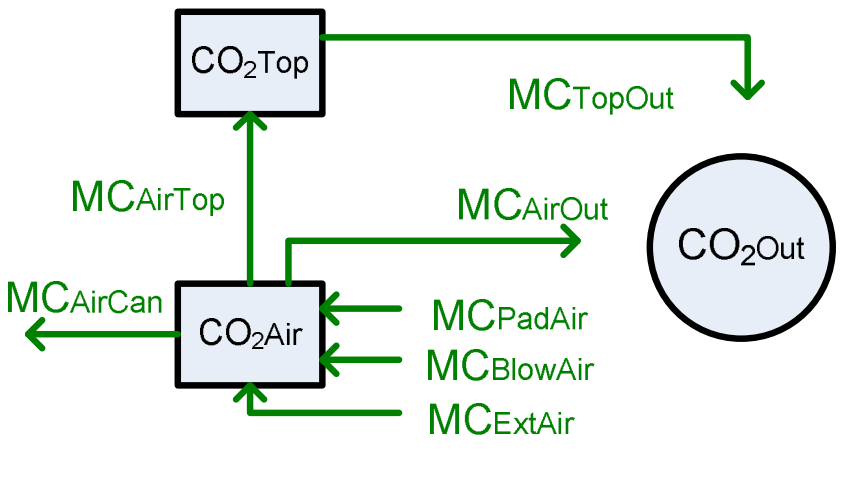
\includegraphics[width=9cm]{CO2}
  \caption{The CO2 flow inside and outside a greenhouse}\label{fig:CO2}
\end{figure}

\begin{itemize}
  \item \(Top/Air\): the compartment above/below the thermal screen
  \item	\(Out/Ext\): outside the greenhouse/external source
  \item \(Blow/Pad\): the direct air heater/pad and fan
  \item \(Can\): the canopy inside the greenhouse
  \item \(MC_{AB}\): the net \(CO_2\) flux from A to B.
\end{itemize}


%%%%%%%%%%
\subsubsection{Dynamical system models and assumptions}
In this section, a dynamical system representing the \(CO_2\) concentration in the greenhouse will be discussed. From figure~\ref{fig:CO2}, the fluctuation of \(CO_2\) concentration in the lower and upper compartments of the greenhouse is represented by two differential equations.
\begin{equation}
  \begin{cases}
    cap_{CO_2 Air}\dot{CO_{2 Air}} = MC_{BlowAir} + MC_{ExtAir} + MC_{PadAir} \\ \qquad \qquad \qquad \qquad \qquad
    - MC_{AirCan} - MC_{AirTop} - MC_{AirOut}                                 \\
    cap_{CO_2 Top}\dot{CO_{2 Top}} = MC_{AirTop} - MC_{TopOut}
  \end{cases}
\end{equation}
\begin{itemize}
  \item \(cap_{CO_{2Top/Air}}\): capacity of the compartment above/below the thermal screen to store \(CO_2\) (m)
  \item	\(CO_{2Top/Air}\): the rate change of \(CO_2\) concentration in the compartment above/below the thermal screen in time \((mg\;m^{-3}\;s^{-1})\);
  \item \(MC_{AB}\): the net \(CO_2\) flux from A to B \((mg\;m^{-2}\;s^{-1})\)
\end{itemize}


In order to solve the equations, we must consider the formulas that calculate each \(MC_{AB}\) that was presented.

Here are formulas to calculate \(MC_{AB}\). First, we consider the amount of \(CO_2\) going from the heater into the greenhouse air as follows.

\begin{gather}
  MC_{BlowAir} ={\eta_{HeatCO_2}}H_{BlowAir} =\frac{\eta_{HeatCO_2}U_{Blow}}{A_{Flr}}
\end{gather}
\begin{itemize}
  \item \({\eta_{HeatCO_2}}\): the amount of \(CO_2\) released when 1 Joule sensible energy is produced by the direct air heater \((mg_{CO_2}\;J^{-1})\);	
  \item \(H_{BlowAir}\): the heat flux from the direct air heater to the greenhouse air  \((W\;m^{-2})\);
  \item\(U_{Blow}\): the control valve of the direct air heater ranging in \([0,1]\);
    \item\(Blow\): the heat capacity of the direct air heater \(W\);
    \item \(AFlr\): the area of the greenhouse floor \(m^2\).
\end{itemize}

Similarly, the amount of \(CO_2\) that is pumped into the greenhouse by the third party equals the third party's ability to pump \(CO_2\) \(\phi_{ExtCO_2}\) \((mg\;s^{-1})\) times the dimensionless parameter \(U_{ExtCO_2}\), then divided by the area of the greenhouse.
\begin{gather}
  MC_{ExtAir} = \frac{U_{ExtCO_2}\phi_{ExtCO_2}}{A_{Flr}}
\end{gather}

On the other hand, the amount of \(CO_2\) that enters the greenhouse through the pad system is calculated differently.
It depends on the difference between the concentration of \(CO_2\) inside and outside the greenhouse, and the ability of the pad system for the air to go through. Furthermore, the pad can be adjusted to let in more air. The following formula is used to calculate \( MC_{PadAir}\).

\begin{equation}
  \begin{split}
    MC_{PadAir} & = f_{Pad} (CO_{2 Out} - CO_{2 Air}) \\
    & = \frac{U_{Pad} \phi_{Pad}}{A_{Flr}} (CO_{2 Out} - CO_{2 Air})
  \end{split}
\end{equation}
\begin{itemize}
  \item \(f_{Pad}\): the ventilation flux due to the pad and fan system \((m^{-1})\)
  \item \(U_{Pad}\): the control valve of the pad and fan system ranging in \([0,1]\);
  \item \(\phi_{Pad}\): the capacity of the air flux through the pad \((m^3\;s^{-1})\) 

\end{itemize}
The net flux of \(CO_2\) from the lower compartment to the upper compartment of the greenhouse is more complicated.
It depends on the difference in temperature and air density between the two compartments and the airflow rate through the thermal screen \(f_{ThScr}\) \((m\;s^{-1})\).
\begin{gather}
  MC_{AirTop} = f_{ThScr} (CO_{2 Air} - CO_{2 Top})
\end{gather}

Furthermore, \(f_{ThScr}\) is given by
\begin{gather}
  f_{ThScr} = U_{ThScr} K_{ThScr} |T_{Air} - T_{Top}| ^{\frac{2}{3}} + (1 - U_{ThScr}) {\Bigg[\frac{g(1 - U_{ThScr})W}{2\rho^{Mean}_{Air}} |\rho_{Air} - \rho_{Top}|\Bigg]}^{\frac{1}{2}}
\end{gather}

\begin{itemize}
  \item  \(f_{ThScr}\): the air flux through the thermal screen\((m\;s^{-1})\). 
  \item \(U_{ThScr}\): the control of the thermal screen ranging in \([0,1]\);
  \item \(K_{ThScr}\): the screen flux coefficient determining the permeability of the screen \((m\;K^{-\frac{2}{3}}\;s^{-1})\).
  \item \(g \): the gravitational acceleration \((m\;s^{-2})\).
  \item \(\rho_{Air/Top} \):the density of the greenhouse air below/above the thermal screen \((kg\;m^{-3})\)
  \item \( {2\rho^{Mean}_{Air}}\): the mean density of the greenhouse air \((kg\;m^{-3})\)
  \item \(T_{Air/Top} \): the temperature below/above the thermal screen \(K\)
\end{itemize}

Similarly, for the net \(CO_2\) flux from the inside to the outside of the greenhouse is given by the following formula
\begin{gather}
  MC_{AirOut} = (f_{VentSide} + f_{VentForced})(CO_{2 Air} - CO_{2 Out})
\end{gather}

The flux \(f_{VentSide}\) and \(f_{VentForced}\) \((m s^{-1})\) are respectively the flux due to the fan system on the sidewalls and the fan system inside the greenhouse.

%In this case, we should consider the Bernoulli principle in representing the pressure difference outside and inside of the greenhouse.

\begin{equation} \label{eq:vent_roof_side}
  \begin{split}
    f_{VentRoofSide} & = \frac{C_d}{A_{Flr}} \Bigg[\frac{U^2_{Roof} U^2_{Side} A^2_{Roof} A^2_{Side}}{U^2_{Roof} A^2_{Roof} + U^2_{Side} A^2_{Side}} .\times \frac{2gh_{SideRoof} (T_{Air} - T_{Out})}{T^{Mean}_{Air}} \\
    &\;+ \Bigg(\frac{U_{Roof} A_{Roof} + U_{Side} A_{Side}}{2}\Bigg)^2 + C_W v^2_{Wind} \Bigg]^{\frac{1}{2}}
  \end{split}
\end{equation}
\begin{itemize}
  \item  \(f_{VentRoofSide} \): the ventilation rate through both the roof and side vents \((m s^{-1})\)
  \item  \( C_{d/w}\): discharge/global wind pressure coefficient depending on the greenhouse shape and the use of an outdoor thermal screen \((-)\);
  \item  \(U_{Roof/Side} \): the control of the roof/side openings ranging in \([0,1]\);
  \item  \( A_{Side}\): the roof/side opening area \((m^2)\) .
  \item  \(h_{SideRoof}\): the vertical distance between mid-points of side wall and roof ventilation openings \((m)\)
  \item  \(T^{Mean}_{Air} \): the mean temperature between the indoor and outdoor temperatures \((K)\)
  \item \(v_{Wind} \): wind speed \((m\;s^{-1})\)
\end{itemize}

In the presence of an insect screen, the movement speed of the air currents through the ventilation areas will be reduced by a factor of \(\eta_{InsScr}\), where \(\zeta_{InsScr}\) is the porosity, the ratio of the area of the holes in the screen to the total area of the screen.
\begin{gather}
  \eta_{InsScr} = \zeta_{InsScr} (2 -  \zeta_{InsScr})
\end{gather}

Given the leakage coefficient \(c_{leakage}\), which depends on the greenhouse type and is dimensionless, an amount of approximately half the leakage rate is added to the air-exchange rate, where leakage rate is calculated as below.
\begin{gather}
  f_{leakage} = \begin{cases}
    0.25 \times c_{leakage}     & \text{if} v_{Wind} < 0.25    \\
    v_{Wind} \times c_{leakage} & \text{if} v_{Wind} \geq 0.25
  \end{cases}
\end{gather}

Let \(\eta_{Side\_Thr}\) be the Stack-effect threshold. If \(\eta_{Side}\), the ratio between the sidewalls ventilation
area and the total ventilation area, exceeds the threshold, the Stack effect does not occur and vice versa. Then, \(f_{VentSide}\) is given by the following
\begin{gather}
  f_{VentSide} =
  \begin{cases}
    \eta_{InsScr} f''_{VentSide} + 0.5f_{leakage} & \text{if} \eta_{Side} \geq \eta_{Side\_Thr} \\
    \begin{split}
      & \eta_{InsScr} [U_{ThScr}f''_{VentSide} + \\
      & (1-U_{ThScr})f_{VentRoofSide} \eta_{Side}] + 0.5 f_{leakage}
    \end{split}                    & \text{if} \eta_{Side} < \eta_{Side\_Thr}
  \end{cases}
\end{gather}

In which,  \(f''_{VentSide}\) is  \(f_{VentSide}\) when \(A_{Roof} = 0\).
Moreover, the Stack effect does not occur where is covered by the thermal screen.

The flux \(f_{VentForced}\) by the fan system inside the greenhouse is calculated as follows.
\begin{gather}
  f_{VentForced} = \frac{\eta_{InsScr} U_{VentForced} \phi_{VentForced} } {A_{Flr}}
\end{gather}

The dimensionless parameter \(U_{VentForced} \in [0,1]\) is to adjust the wind speed \(\phi_{VentForced}\) due to
the system \((m^3\;s^{-1})\).

Similarly to \(MC_{AirOut}\), the net \(CO_2\) flux from the greenhouse to outside the greenhouse through the roof openings is calculated by using the formula below, where \(f_{VentRoof}\) is the flux rate through the roof openings.
\begin{gather}
  MC_{TopOut} = f_{VentRoof}(CO_{2 Top} - CO_{2 Out})
\end{gather}

\(f_{VentRoof}\) is the flux rate openings and is given by
\begin{gather}
  f_{VentRoof} =
  \begin{cases}
    \eta_{InsScr} f''_{VentRoof} + 0.5f_{leakage} & \text{if} \eta_{Roof} \geq \eta_{Roof\_Thr} \\
    \begin{split}
      & \eta_{InsScr} [U_{ThScr}f''_{VentRoof} + \\
      & (1-U_{ThScr})f_{VentRoofSide} \eta_{Side}] + 0.5 f_{leakage}
    \end{split}                    & \text{if}  \eta_{Roof} < \eta_{Roof\_Thr}
  \end{cases}
\end{gather}

% check again part
However, when the ratio of the roof-opening area to the total ventilation area exceeds the Stack-effect threshold, the Stack effect does not occur and we cannot reuse the formula~\ref{eq:vent_roof_side} where \(A_{Side} = 0\) to
calculate \(f''_{VentRoof}\).
\begin{gather}
  f''_{VentRoof} = \frac{C_d U_{Roof} A_{Roof}}{2A_{Flr}} {\Big[\frac{gh_{Roof}(T_{Air} - T_{Out})}{2T^{Mean}_{Air}} + C_w v^2_{Wind} \Big]}^{ \frac{1}{2}}
\end{gather}

Finally, we need to consider the amount of \(CO_2\) absorbed into the leaves due to photosynthesis.
\begin{gather}
  MC_{AirCan} = M_{CH_2O} h_{C_{Buf}} (P - R)
\end{gather}
Here, 
\begin{itemize}
  \item  \( M_{CH_2O} \):the molar mass of \(CH_2O\) \((mg\;\mu mol^{-1})\)
  \item  \( P\): the photosynthetic rate \((\mu mol_{CO_2}\;m^{-2}\;s{-1})\)
  \item  \(R\):  the respiration rate \((\mu mol_{CO_2}\;m^{-2}\;s^{-1})\)
  \item  \( h_{C_{Buf}}\):shows the cessation of photosynthesis when \(CH_2O\) is \(C_{Buf}\) \((mg\;m^{-2})\) has reached \(C_{Max}\) \((mg\;m^{-2})\), which is the limit of the carbohydrates storage of the plants. The respiration rate during this process is usually as about \(1\%\) of the photosynthesis rate, and thus can be omitted during further calculation. The photosynthesis rate is described in more detail in Chapter 4.
 
\end{itemize}

%%%%%%%%%%%


\subsubsection{Photosynthesis of C3 plants}
\setcounter{equation}{19}
Photosynthesis, the process by which green plants and certain other organisms transform light energy into chemical energy. During photosynthesis in green plants, light energy is captured and used to convert water, carbon dioxide, and minerals into oxygen and energy-rich organic compounds.

Photosynthesis has two phases consisting of the light-dependence phase and the light-independence (or dark) phase.

The photosynthetic rate \(P\) is defined as the diffusion of \(CO_2\) from air into the leaf cells through stomata. From Fick's law for gas diffusion, we construct:
\begin{gather}
  P = \frac{CO_{2Air} - CO_{2Stom}}{Res}
\end{gather}

The notation \(CO_{2Stom}\) is the concentration of CO2 in the stomata \((\mu mol\;m^{-3})\) and \(Res\) is the resistance-to-absorption coefficient \((s\;m^{-1})\), this coefficient of resistance depends on many factors including the speed of the wind blowing through the leaves.

This way of calculating photosynthetic rate \(P\) is different from the model of Vanthoor 2011. In there the author uses:

\begin{gather}
  P = \frac{J \cdot (CO_{2Stom} - \Gamma)}{4 \cdot (CO_{2Stom} + 2\Gamma)}
\end{gather}

where \(J\) \((\mu mol \{e^-\} m^{-2} s^{-1})\) is the electron transport rate, 4 \((\mu mol \{e^-\} \mu mol^{-1} \{CO2\})\) is the
number of electrons per fixed \(CO_2\) molecule, \(CO_{2Stom}\) \((\mu mol\{CO_2\}\;mol^{-1}\{air\})\) is the \(CO_2\) concentration in the stomata and \(\Gamma\) \((\mu mol \{CO_2\} mol^{-1} \{air\})\) is the \(CO_2\) compensation point.

Following by the photorespiration \(R\):
\begin{gather}
  R = P \cdot \frac{\Gamma}{CO_{2Stom}}
\end{gather}

But since we do not consider electron transport rate, we will use equation $(20)$ constructed from Fick's law combined with Michaelis-Menten model.

In the dark phase, through Michaelis-Menten relationship describing enzyme-substrate reaction, the photosynthetic rate is given by:
\begin{gather}
  P = \frac{P_{Max} \cdot CO_{2Stom}}{CO_{2 0.5} + CO_{2Stom}}
\end{gather}
where\(P_{Max}\) is the photosynthesis rate at saturating \(CO_{2Stom}\) and \(CO_{2 0.5}\) is the concentration of \(CO_2\) in the substrate when \(P = P_{Max}/2\) \((\mu mol\;m^{-3})\).

 We form a quadratic equation for the rate of photosynthetic \(P\). The photosynthetic rate \(P\) then no longer depends on the concentration of \(CO_2\) in the stomata but only on the concentration of \(CO_2\) in the air, the resistance coefficient Res, and the maximum photosynthetic rate.
\begin{gather}
  ResP^2 - (CO_{2Air} + CO_{2 0.5} + ResP_{Max})P + CO_{2Air}P_{Max} = 0
\end{gather}

Solving equation $(22)$ requires the maximum rate of photosynthesis needs to be determined. For the model for the photosynthesis of one leaf unit, the maximum photosynthetic rate is usually be found through the Arrhenius model.
\(P_{Max}\) and the Arrhenius model:
\begin{gather}
  k(T) = k(T_0)e^{-\frac{H_a}{R}(\frac{1}{T} - \frac{1}{T_0})}
\end{gather}
\begin{itemize} 
  \item \( T\):the temperature of the leaf \( K\)
  \item \( T_0\):a specific temperature of the leaf that we know the reaction rate \( K\)
  \item \(k(T) \):the reaction rate \((-)\);
  \item \( H_a\):the activation energy \((J\;mol^{-1})\),
  \item \( R\):the ideal gas constant \((J\;mol^{-1})\;K^{-1}\),
\end{itemize}



Yet a problem is raised when the temperature increases to a certain threshold, the enzyme activity will be inhibited and the photosynthesis is slowed down and cease to advance. A model represents the activity of the Rubisco enzyme during photosynthesis with temperature as its parameter.
\begin{gather}
  f(T) = \frac{1 + e^{-\frac{H_d}{R}( \frac{1}{T_0} - \frac{1}{\frac{H_d}{S}} )}}{1 + e^{-\frac{H_d}{R}(\frac{1}{T} - \frac{1}{\frac{H_d}{S}})}}
\end{gather}
In the model $(24)$, \(f(T)\) represents the enzyme activity at \(T(K)\), \(H_d\) is the deactivation energy \((J\;mol^{-1})\), and \(S\) is the corresponding entropy quantity \((J\;mol^{-1}\;K^{-1})\).

Combining $(23)$ and $(24)$, we obtain the formula for maximum rate of photosynthetic rate.
\begin{gather}
  P_{Max}(T) = k(T)f(T)
\end{gather}

For a photosynthesis for the whole canopy, considering \(LAI\) (leaf area index), due to Beer's law, the intensity of the transmitted beam \(I\) with the initial state is \(I_0\) \((\mu mol\{photons\}\;m^{-2}\;s^{-1})\) is equal to
\begin{gather}
  I = \frac{I_0.K.e^{-K.LAI}}{1 - m}
\end{gather}

If the leaves are horizontally stratified such as in the case of tomato, the dimensionless extinction coefficient \(K\) will be between 0.7 and 1.0. Meanwhile, if the leaves are sloping as in the case of wet rice, \(K\) will be between 0.3 and 0.5. \(m\) is the transmittance coefficient of the leaves which is set as 0.1.

The amount of light absorbed by the canopy can be measured as the difference in the intensity of the light ray before entering the foliage and after passing through the foliage
\begin{gather}
  L =L_0(1 - \frac{K.e^{-K.LAI}}{1 - m})
\end{gather}

In this formula, L is luminous flux received by the leaves per unit area of the greenhouse floor \((\mu mol\{photons\}\;m^{-2}\;s^{-1})\) and \(L_0\) is the initial value of L.

For calculating the maximum photosynthetic rate of all leaves in the greenhouse, we apply the modified Arrhenius model.
\begin{gather}
  k(T) = LAI \cdot k(T_0) \cdot e^{-\frac{H_a}{R}(\frac{1}{T} - \frac{1}{T_0})}
\end{gather}
\begin{itemize}
  \item \(T\):the temperature of the canopy \(K \)
  \item \(T_0\): a specific temperature of the canopy that we know the reaction rate \(K \)
  \item \(k(T)\): the reaction rate of the canopy at \( T (-)\)
  \item \(k(T_0)\): the reaction rate in the stroma of a leaf at \( T_0 (-)\)
\end{itemize}

Unlike the photosynthesis model for one leaf unit, the amount of light energy absorbed into the foliage in response to \(LAI\) needs to be added since it affects the maximum photosynthetic rate \(P_{Max}\). Therefore, we consider the following formula of \(P_{Max}\), which is a dependent function on \(L\) and \(T\).
\begin{gather}
  P_{Max} (L,T) = \frac{P_{MLT} \cdot P_{Max}(T) \cdot L}{L + L_{0.5}}
\end{gather}


In which, 
\begin{itemize}
 \item \( L\): the photosynthetically active radiation absorbed by the canopy\((\mu mol\{photons\}\;m^{-2}\;s^{-1})\)
 \item \(L_{0.5}\): the photosynthetically active radiation at which \(P_{Max} (L,T) = P_{Max}(T)/2\) \((\mu mol\{photons\}\;m^{-2}\;s^{-1})\)
 \item \(P_{MLT}\): the value of \(P_{Max}\) at saturation L and optimum T \((\mu mol\{CO_2\}\;m^{-2}\;s^{-1})\)
\end{itemize}
%%%%%%%%%

\subsubsection{Vanthoor 2011 model of photosynthesis}
For calculating photosynthesis rate and respiration rate, we we will use Equation (9.10) and relevant ones in reference [Van11].

Photosynthesis rate at canopy level, P, is described by (Farquhar, 1988):
\begin{align}
  P = \frac{J \cdot (CO_{2Stom} - \Gamma)}{4 \cdot (CO_{2Stom} + 2\Gamma)}
\end{align}
where \(J\) (\(\mu mol\{e^-\}\ m^{-2}\ s^{-1}\)) is the electron transport rate, \(4\) (\(\mu mol \{e^-\}\ \mu mol^{-1} \{CO_2\}\)) is the number of electrons per fixed \(CO_2\) molecule, \(CO_{2Stom}\) (\(\mu mol\{CO_2\}\ mol^{-1}\{air\}\)) is the \(CO_2\) concentration in the stomata and \(\Gamma\) (\(\mu mol \{CO_2\}\ mol^{-1} \{air\}\)) is the \(CO_2\) compensation point.

The photorespiration, R, is described by (Farquhar \& Von Caemmerer, 1982):
\begin{align}
  R = P \cdot \frac{\Gamma}{CO_{2Stom}} 
\end{align}

The electron transport rate, J, is a function of the potential rate of electron transport and of the absorbed PAR by the canopy (Farquhar, 1988; Evans \& Farquhar, 1991):

\begin{align}
  J = \frac{J^{POT} + \alpha PAR_{can} - {\sqrt{(J^{POT} + \alpha PAR_{can})}^2 - 4\Theta\cdot J^{POT}\cdot \alpha PAR_{can}}}{2 \Theta}
\end{align}
where \(J^{POT}\) (\(\mu mol\{e^-\}\ m^{-2}\ s^{-1}\)) is the potential rate of electron transport, \(PAR_{Can}\) (\(PAR\) by the canopy) (\(\mu mol\{photons\}\ m^{-2}\ s^{-1}\)) is the absorbed \(PAR\), \(\alpha\) (\(\mu mol\{e^-\}\ \mu mol^{-1}\{photons\}\)) is the conversion factor from photons to electrons, including an efficiency term, and \(\Theta\) (\(-\)) is the degree of curvature of the electron transport rate.

The potential rate of electron transport POT J , depends on temperature (Farquhar et al., 1980):

\begin{align}
  J^{POT} = J^{MAX}_{25,Can} \cdot \exp \left(E_j\frac{T_{Can,K}-T_{25,K}}{R\cdot T_{Can,K}\cdot T_{25,K}}\right) \cdot \frac{1 + \exp \left(\frac{S\cdot T_{25,K}-H}{R\cdot T_{25,K}}\right)}{1 + \exp \left(\frac{S\cdot T_{Can,K}-H}{R\cdot T_{Can,K}}\right)}
\end{align}
where \(J^{MAX}_{25,Can}\) (\(\mu mol \{e^-\}\ m^{-2}\ s^{-1}\)) is the maximum rate of electron transport at \(25 \celsius\) for the canopy, \(E_j\) (\(J\ mol^{-1}\)) is the activation energy for \(J^{POT}\), \(T_{Can,K}\) (\(K\)) is the canopy temperature, \(T_{25,K}\) (\(K\)) is the reference temperature at \(25 \celsius\), \(R\) (\(J\ mol^{-1}\ K^{-1}\)) is the molar gas constant, \(S\) (\(J\ mol^{-1}\ K^{-1}\)) is the entropy term and \(H\) (\(J\ mol^{-1}\)) is the deactivation energy.

The maximum rate of electron transport at 25°C for the canopy is calculated by (Evans \& Farquhar, 1991):

\begin{align}
  J^{MAX}_{25,Can} = LAI \cdot J^{MAX}_{25,Leaf}
\end{align}
where \(J^{MAX}_{25,Leaf}\), (\(\mu mol\{e^-\}\ m^{-2}\{leaf\}\ s^{-1}\)) is the maximum rate of electron transport for the leaf at \(25 \celsius\).\\


\textbf{In this exercise with assumption that \(PAR_Can\) is a constant}\\
The total PAR absorbed by the canopy is the sum of the PAR transmitted by the greenhouse
cover that is directly absorbed, and the PAR reflected by the greenhouse floor that is
indirectly absorbed:
\begin{align}
  PAR_{Can} = PAR_{GhCan} + PAR_{FlrCan}
\end{align}

The \(PAR\) which is directly absorbed by the canopy is described by a negative exponential decay of light with \(LAI\) in a homogeneous crop (Ross, 1975):
\begin{align}
  PAR_{GhCan} = PAR_{Gh}\cdot (1-\rho_{can})\cdot(1 - \exp \left(-K_1\cdot LAI\right))
\end{align}
where \(PAR_{Gh}\) (\(\mu mol \{photons\}\ m^{-2}\ s^{-1}\)) is the \(PAR\) above the canopy, \(\rho_{can}\) (\(-\)) is the reflection coefficient of the canopy for \(PAR\) and \(K_1\) is the extinction coefficient of the canopy for \(PAR\) (\(-\)).

The PAR above the canopy is described by:
\begin{align}
  PAR_{Gh} = \tau_{Gh} \cdot \eta_{Glob\_PAR}\cdot I_{Glob}
\end{align}
where \(\tau_{Gh}\) (\(-\)) is the light transmission of the greenhouse cover \(\eta_{Glob\_PAR}\) (\(\mu mol\{photons\}\ J^{-1}\)) is a conversion factor from global radiation to \(PAR\) and \(I_{Glob}\) (\(W\ m^{-2}\)) is the outside global radiation.

Absorption of \(PAR\) reflected by the greenhouse floor is described by:
\begin{align}
  PAR_{FlrCan} = \rho_{Flr}PAR_{Gh}\cdot (1-\rho_{Can})\cdot \exp \left(K_1\cdot LAI\right) \cdot (1 - \exp \left(K_2\cdot LAI\right))
\end{align}
where \(\rho_{Flr}\) (\(-\)) is the reflection coefficient of the greenhouse floor and \(K_2\) (\(-\)) is the extinction coefficient of the canopy when \(PAR\) is reflected from the floor to the canopy. We assumed \(K_2\) to be equal to \(K_1\).

The CO2-concentration inside the stomata, CO2Stom depends on the stomatal and mesophyl conductance, boundary layer resistance, the photosynthesis rate and the difference between the CO2-concentration in the stomata and the CO2-concentration of the greenhouse air. However, the CO2-concentration in the stomata is assumed to be a fixed fraction of the CO2-concentration in the greenhouse air (Evans \& Farquhar, 1991):

\begin{align}
  CO_{2Stom} = \eta_{CO_{2Air\_Stom}} \cdot CO_{2Air}
\end{align}
where \(\eta_{CO_{2Air\_Stom}}\) is conversion factor from the \(CO_2\) concentration of the greenhouse air, \(CO_{2Air}\), to the \(CO_2\) concentration in the stomata.(Evans \& Farquhar, 1991).

The \(CO_2\) compensation point (\(\Gamma\)) affects the leaf photosynthesis rate and depends on temperature (Farquhar 1998) . To avoid unrealistically low optimal canopy temperatures, the sensitivity of the compensation point to temperature was adjusted by making the slope dependent of the ratio of \(J^{MAX}_{25,Leaf}\) and \(J^{MAX}_{25,Can}\):
\begin{align}
  \Gamma = \frac{J^{MAX}_{25,Leaf}}{J^{MAX}_{25,Can}}c_{\Gamma} T_{Can} + 20 c_{\Gamma} \left(1-\frac{J^{MAX}_{25,Leaf}}{J^{MAX}_{25,Can}}\right)
\end{align}
where \(c_{\Gamma}\) (\(\mu mol\{CO2\}\ mol^{-1}\{air\}\ K^{-1}\)) determines the effect of canopy temperature on the \(CO_2\) compensation point.






%%%%%%%%%%%%%%%%%%%%%%%%%%%%%%%%%
\subsection{Implementing the code} 
\begin{itemize}
  \item Two differential equations represents the fluctuation of $\{CO_2\}$ concentration:
        \begin{multline*}
          cap_{CO_{2Air}}\dot{CO_{2Air}} = MC_{BlowAir} + MC_{ExtAir} + MC_{PadAir} \\
          - MC_{AirCan} - MC_{AirTop} - MC_{AirOut} ~~~~ [mg\;m^{-2}\;s^{-1}]
        \end{multline*}
        \begin{multline*}
          cap_{CO_{2Top}}\dot{CO_{2Top}} = MC_{AirTop} - MC_{TopOut} ~~~~~~~~~~~~~~~~~~~~~~~~~~~~ [mg\;m^{-2}\;s^{-1}]
        \end{multline*}
\end{itemize}
All of the MC formula we need are demonstrated as below:\\
\begin{itemize}
\item $MC_{BlowAir} = \frac{\eta_{HeatCO_2}U_{Blow}}{A_{Flr}}$

\begin{mdframed}[leftline=false,rightline=false,backgroundcolor=cyan!10]
  \begin{minted}[linenos,breaklines,breaksymbolleft=,obeytabs=true,tabsize=2]{Python}
def MC_blow_air():    #                 (2.2)
    return (n_heat_Co2 * U_blow * P_blow)/A_flr   
  \end{minted}
\end{mdframed}
\item $ MC_{ExtAir} = \frac{U_{ExtCO_2}\phi_{ExtCO_2}}{A_{Flr}}$
\begin{mdframed}[leftline=false,rightline=false,backgroundcolor=cyan!10]
  \begin{minted}[linenos,breaklines,breaksymbolleft=,obeytabs=true,tabsize=2]{Python}
def MC_ect_air():     #                (2.3)
    return (U_ext_Co2 * third_party_ability)/A_flr
  \end{minted}
\end{mdframed}
\item $ MC_{PadAir} = f_{Pad} (CO_{2 Out} - CO_{2 Air}) \\\\
     = \frac{U_{Pad} \phi_{Pad}}{A_{Flr}} (CO_{2 Out} - CO_{2 Air})$
\begin{mdframed}[leftline=false,rightline=false,backgroundcolor=cyan!10]
  \begin{minted}[linenos,breaklines,breaksymbolleft=,obeytabs=true,tabsize=2]{Python}
def MC_pad_air():    #               (2.4)
    f_pad = (U_pad * ability_airflow)/A_flr
    return f_pad * (Co2_out - Co2_air)            
  \end{minted}
\end{mdframed}
\item $   MC_{AirTop} = f_{ThScr} (CO_{2 Air} - CO_{2 Top})$\\
In order to calculate $MC_{AirTop}$, we need to find the value of $f_{ThScr}$ first:
\begin{mdframed}[leftline=false,rightline=false,backgroundcolor=cyan!10]
  \begin{minted}[linenos,breaklines,breaksymbolleft=,obeytabs=true,tabsize=2]{Python}
def p_air_average():
    temp = (g * M_air * h_elevation)/(293.15 * R)
    return (p_air_average_0 * math.exp(temp))
#?print(p_air_average())
def f_Th_Scr():      #                   (2.6)
    diff_T = abs(T_air - T_top) ** (2.0/3.0)
    diff_p = abs(p_air - p_top)
    left_part = (((g * (1.0 - U_Th_Scr)) / (p_air_average() * 2.0)) * diff_p) ** (1.0/2.0)
    return (U_Th_Scr * K_Th_Scr * diff_T) + ((1.0 - U_Th_Scr) * left_part)
  \end{minted}
\end{mdframed}
\begin{mdframed}[leftline=false,rightline=false,backgroundcolor=cyan!10]
  \begin{minted}[linenos,breaklines,breaksymbolleft=,obeytabs=true,tabsize=2]{Python}
def MC_air_top():    #            (2.5)
    return f_Th_Scr() * (Co2_air - Co2_top)
  \end{minted}
\end{mdframed}
\item $ MC_{AirOut} = (f_{VentSide} + f_{VentForced})(CO_{2 Air} - CO_{2 Out})$

\(f_{VentSide}\) is calculated in the separated function as below:
\begin{mdframed}[leftline=false,rightline=false,backgroundcolor=cyan!10]
  \begin{minted}[linenos,breaklines,breaksymbolleft=,obeytabs=true,tabsize=2]{Python}
def f_Vent_roof_side(): #* equation 10            (2.8)
    first_part = ((U_roof * U_side * A_side * A_roof) ** 2.0)/(((U_roof**2.0) * (A_roof**2)) + ((U_side**2.0) * (A_side**2)))
    second_part = (2.0 * g * h_side_roof * (T_air-T_out))/T_average_air
    third_part = (((U_roof * A_roof) + (U_side * A_side))/2.0) ** 2.0
    return (C_d * (((first_part * second_part) + (third_part * C_w * (v_wind ** 2.0))) ** (1.0/2.0)))/A_flr
  \end{minted}
\end{mdframed}
\begin{mdframed}[leftline=false,rightline=false,backgroundcolor=cyan!10]
  \begin{minted}[linenos,breaklines,breaksymbolleft=,obeytabs=true,tabsize=2]{Python}
def n_ins_scr(): #*equation 11             (2.9)
    return dimensionless_ins_scr * (2.0 - dimensionless_ins_scr)
#?print(n_ins_scr())
  \end{minted}
\end{mdframed}
\begin{mdframed}[leftline=false,rightline=false,backgroundcolor=cyan!10]
  \begin{minted}[linenos,breaklines,breaksymbolleft=,obeytabs=true,tabsize=2]{Python}
def f_leak_age(): #*equation 12             (2.10)
    return 0.25 * c_leak_age if v_wind < 0.25 else v_wind * c_leak_age
#?print(f_leak_age())
  \end{minted}
\end{mdframed}

\begin{mdframed}[leftline=false,rightline=false,backgroundcolor=cyan!10]
  \begin{minted}[linenos,breaklines,breaksymbolleft=,obeytabs=true,tabsize=2]{Python}
def f_Vent_side(): #*equation 13             (2.11)
    if n_side >= n_side_thr :
        return (n_ins_scr() * f_2time_derivative_Vent_side() + 0.5 * f_leak_age())
    else :
        return (n_ins_scr() * (U_Th_Scr * f_2time_derivative_Vent_side() + (1.0 - U_Th_Scr) * f_Vent_roof_side()) + 0.5 * f_leak_age())
#?print(f_Vent_side())
  \end{minted}
\end{mdframed}

The value of \(f_{VentForced}\) is calculated as below:
\begin{mdframed}[leftline=false,rightline=false,backgroundcolor=cyan!10]
  \begin{minted}[linenos,breaklines,breaksymbolleft=,obeytabs=true,tabsize=2]{Python}
def f_Vent_forced(): #*equation 14             (2.12)
    return (n_ins_scr() * U_Vent_forced * the_wind_speed)/A_flr
#?print(f_Vent_forced())
  \end{minted}
\end{mdframed}

The value of two variable \(f_{VentSide}\) and \(f_{VentForced}\) are calculated so we can get calculate \(MC_{AirOut}\) through the formula:
\begin{mdframed}[leftline=false,rightline=false,backgroundcolor=cyan!10]
  \begin{minted}[linenos,breaklines,breaksymbolleft=,obeytabs=true,tabsize=2]{Python}
def MC_air_out(): #* equation 9               (2.7)
    return ((f_Vent_side() + f_Vent_forced()) * (Co2_air - Co2_out))
#?print(MC_air_out())  
\end{minted}
\end{mdframed}

\item $MC_{TopOut} = f_{VentRoof}(CO_{2 Top} - CO_{2 Out})$\\ 
Calculate the $f_{VentRoof}$:
\begin{mdframed}[leftline=false,rightline=false,backgroundcolor=cyan!10]
  \begin{minted}[linenos,breaklines,breaksymbolleft=,obeytabs=true,tabsize=2]{Python}
def f_2time_derivative_Vent_roof(): #* equation 17       (2.15)
    first = (C_d * U_roof * A_roof) / (2.0 * A_flr)
    second = (g * h_Vent * (T_air - T_out)) / (2.0 * T_average_air)
    return first * ((second + C_w * (v_wind ** 2.0)) ** (1.0/2.0))
#?print(f_2time_derivative_Vent_roof())

def f_Vent_roof(): #* equation 16     (2.14)
    if n_roof >= n_roof_thr:
        return (n_ins_scr() * f_2time_derivative_Vent_roof() + 0.5 * f_leak_age())
    else:
        return (n_ins_scr() * (U_Th_Scr * f_2time_derivative_Vent_roof() + (1 - U_Th_Scr) * f_Vent_roof_side() * n_side) + 0.5 * f_leak_age())
#?print(f_Vent_roof())
\end{minted}
\end{mdframed}
$MC_{TopOut}$ is calculated through the $f_{VentRoof}$
\begin{mdframed}[leftline=false,rightline=false,backgroundcolor=cyan!10]
  \begin{minted}[linenos,breaklines,breaksymbolleft=,obeytabs=true,tabsize=2]{Python}
def MC_top_out(): #*equation 15                   (2.13)
    return (f_Vent_roof() * (Co2_top - Co2_out))
\end{minted}
\end{mdframed}
\item $MC_{AirCan} = M_{CH_2O} h_{C_{Buf}} (P - R)$
All the variables that necessary to calculate P and R are determined as:
\begin{mdframed}[leftline=false,rightline=false,backgroundcolor=cyan!10]
  \begin{minted}[linenos,breaklines,breaksymbolleft=,obeytabs=true,tabsize=2]{Python}
def J_Pot(): #* equation 9.15               (2.35)
    first_power =  (E_j * (T_can_k - T_25_k)) / (R * T_25_k * T_can_k)
    second_power = (S * T_25_k - H) / (R * T_25_k)
    third_power = (S * T_can_k - H) / (R * T_can_k) 
    return (L_a_i * J_max_25_leaf * math.exp(first_power) * (1 + math.exp(second_power)))/(1 + math.exp(third_power))
#?print(J_Pot())

conversion_factor = 0.385
degree_of_curvature = 0.7
def J(): #* equation 9.14                 (2.34)
    sqrt_side = ((J_Pot() + (conversion_factor * PAR_can())) ** 2.0) - 4.0 * degree_of_curvature * J_Pot() * PAR_can() * conversion_factor
    return (J_Pot() + conversion_factor * PAR_can() - math.sqrt(sqrt_side))/(2.0 * degree_of_curvature)
#?print(J())

n_Co2_air_stom = 0.67
c_Co2_compensation_point = 1.7

def Co2_stom(): #* equation 9.21            (2.41)
    return n_Co2_air_stom * Co2_air
def Co2_compensation_point(): #* equation 9.22 
    return c_Co2_compensation_point * T_can_k

def P():                      (2.32)
    return (J() * (Co2_stom() - Co2_compensation_point()))/(4.0 * (Co2_stom() + (2.0 * Co2_compensation_point())))
def R():                     (2.33) 
    return (P() * Co2_compensation_point())/Co2_stom()
\end{minted}
\end{mdframed}
After find all the variables, we calculate $MC_{AirCan}$
\begin{mdframed}[leftline=false,rightline=false,backgroundcolor=cyan!10]
  \begin{minted}[linenos,breaklines,breaksymbolleft=,obeytabs=true,tabsize=2]{Python}
def MC_air_can(): #*equation 18        (2.16)
    return M_ch2o * h_C_Buf * (P() - R())
#?print(MC_air_can())
\end{minted}
\end{mdframed}
\end{itemize}

In the end, we find $\dot{CO_{2Air}}$ and $\dot{CO_{2Top}}$ as dx function with parameter x are $CO_{2Air}$ and $CO_{2Top}$. The rate of concentration of $CO_2$ is calculated by dividing the right side of formula (sum of all MC stuff) by $cap_{CO_2Air}$ and $cap_{CO_2Top}$ respectively. 


\section{Implement the program}
	\subsection{Data}
In this assignment, we consider the statistic in the greenhouse model in Texas, USA. According to the statistic in table 8.2 in \emph{A model based greenhouse design} reference, we have:
\begin{itemize}
    \item $cap_{CO2Air}$ equal to the value of height of the greenhouse compartment below the thermal screen, which is 4.7(m)
    \item $cap_{CO2Top}$ equal to the value of height of the greenhouse compartment above the thermal screen, which means the subtraction of mean height of greenhouse and the height below the screen equal to 5.1 - 4.7 = 0.4 (m)
    \item $n_{heatCO2}$ = 0.057 ($mgCO_2J^{-1}$)
    \item $U_{Blow}$ is a random value between 0 and 1.
    \item $P_{Blow}$ = 0 (W)
    \item $A_{flr}$ = $7.8*10^4$ ($m^2$)
    \item $U_{extCo2}$ is a random value between 0 and 1.
    \item $\phi _{ExtCO_2}$ = $4.3*10^5 (mgs^{-1})$.
    \item $U_pad$ is a random value between 0 and 1.
    \item $\phi pad$ = 0.
    \item $U_{ThSrc}$ is a random value between 0 and 1.
    \item $K_{ThSrc}$ $= 0.25*10^{-3}(m^{3}m^{-2}K^{-0.66}s^{-1})$
    \item $h_{elevation}$ = 1470 (m)
    \item $S_{Insscr}$ = 1.0
    \item $c_{leakage}$ = $10^{-4}$ 
    \item $C_d$ = 0.65
    \item $C_w$ = 0.09
    \item $U_{roof}$ is a random value between 0 and 1.
    \item $A_{roof}$ = 14040
    \item $A_{side}$ = 0
    \item $\eta_{roof}$ = $1.0$
    \item $\eta_{roofThr}$ = 0.9
    
\end{itemize}
Some greenhouse parameters are constant value:
\begin{itemize}
    \item g = $9.81 (ms^{-1})$
    \item R = 8.3145 $(Jmol{-1}K{-1})$
\end{itemize}
Table 4.2 demonstrate the statistic of average outdoor climate
\begin{itemize}
    \item $v_{wind}$ = $2.9 (ms^{-1})$
    \item $T_{out}$ = 23.9 (Celcius) = 297.05K
    \item $T_{aveAir}$ = 20 (Celcius) = 293.15K
\end{itemize}
Some parameters are collected from the statistic in table 9.1 (p.270) in Van11
\begin{itemize}
    \item $M_{CH_2O}$ = $30*10^{-3} (mg{CH2O}µmol^{-1}{CH2O})$
    \item $h_CBuf$ = 1
    \item $h_{Vent}$ = 0.97
    \item $U_{Ventforce}$ is a random number between 0 and 1.
\end{itemize}
From table 8.1 in  in Van11s' book, we have value of some parameters:
\begin{itemize}
    \item $p_{Air0}$ = 1.2 $(kgm^{-3})$. We consider the density at sea level
    \item $M_{Air}$ = 28.9 $(kgkmol^{-1})$
\end{itemize}

According to Val11's book, we have value of some parameters:
\begin{itemize}
    \item 
\end{itemize}


*All the data collected in Van11's book (1991) are precise in times from day 157th to 162th. So the initial value of $CO_2$ Concentration is assumed based on the figure below from Van11 (page 97): 
\begin{figure}[H]
  \centering
  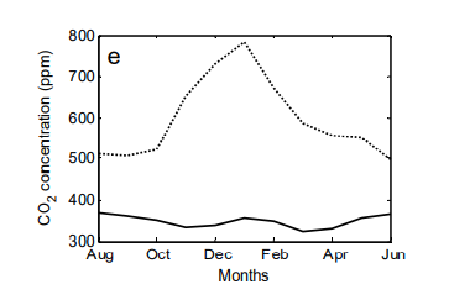
\includegraphics[width=9cm]{CO2Concentration.png}
  \caption{Concentration of $CO_2$}\label{fig:Concentration}
\end{figure}

The picture above witness the CO2 concentration during day period and the in the low-tech greenhouse in Spain (solid line) and in the high-tech
greenhouse in Texas, USA (dotted line) from August 1st to July 1st. Since we just considered the statistic in Texas during the time between 157th and 162th, means that its is between Apr and Jun on the graph.\\

So we assume the initial value of $CO_{2Air}$ and $CO_{2Top}$ below:

\begin{itemize}
    \item $CO_{2Air}$ is 550 (ppm) = 990.005($mgm^{-3}$)
    \item $CO_{2Top}$ is 545 (ppm) = 981.005($mgm^{-3}$)
\end{itemize}

	\subsection{Result}
	\begin{itemize}
\item $MC_{BlowAir} = \frac{\eta_{HeatCO_2}U_{Blow}P_{Blow}}{A_{Flr}}$
\begin{table}[h]
\centering
\begin{tabular}{|l|l|l|l|}
\hline
\rowcolor[HTML]{FFFC9E} 
\textbf{$n_{HeatCO2}$} & \textbf{$U_{Blow}$} & \textbf{$P_{Blow}$}            & \textbf{$A_{flr}$}             \\ \hline
0.057             & 0.52           & 0.0 & 7.8*10\textasciicircum{}4 \\ \hline
\end{tabular}
\end{table}\\
$\rightarrow MC_{BlowAir} = 0.0$ 
\item $ MC_{ExtAir} = \frac{U_{ExtCO_2}\phi_{ExtCO_2}}{A_{Flr}}$
\begin{table}[h]
\centering
\begin{tabular}{|l|l|l|}
\hline
\rowcolor[HTML]{FFFC9E} 
\textbf{$U_{ExtCO2}$} & \textbf{$\phi_{ExtCO2}$}              & \textbf{$A_{flr}$}             \\ \hline
0.39        & 4.3*10\textasciicircum{}5 & 7.8*10\textasciicircum{}4 \\ \hline
\end{tabular}
\end{table}\\
$\rightarrow MC_{ExtAir}  = 2.15$
\item $ MC_{PadAir}  = f_{Pad} (CO_{2 Out} - CO_{2 Air}) 
     = \frac{U_{Pad} \phi_{Pad}}{A_{Flr}} (CO_{2 Out} - CO_{2 Air}) = 0$\\
The $MC_{PadAir}$ equal to zero since greenhouse model in Texas, which do not have the cooling pad system. 
\item $   MC_{AirTop} = f_{ThScr} (CO_{2 Air} - CO_{2 Top})$\\

$f_{ThScr} = U_{ThScr}K_{ThScr}|T_{Air}-T_{Top}|^{\frac{2}{3}}+(1-U_{ThScr})[\frac{g(1-U_{ThScr})}{2\rho_{MeanAir}}|\rho_{Air} - \rho_{Top}|]^{\frac{1}{2}}$
\\
$\rho_{Air}$ = $\rho_{Air0}$$exp(\frac{gM_{Air}h_{Elevation}}{293.15R})$
\begin{table}[H]
\centering
\begin{tabular}{|l|l|l|l|l|}
\hline
\rowcolor[HTML]{FFFC9E} 
\cellcolor[HTML]{FFFC9E}\textbf{$p_{Air}$} & \cellcolor[HTML]{FFFC9E}\textbf{g} & \textbf{$M_{Air}$} & \textbf{$h_{elevation}$} & \textbf{R}                   \\ \hline
1.2                                   & 9.81                               & 28.96         & 1470                & $8.3145*10^3$ \\ \hline
\end{tabular}
\end{table}
$\rho_{Top}$ = $\rho_{Air0}$$exp(\frac{gM_{Air(}h_{Elevation}+h_{Air})}{293.15R})$
\begin{table}[H]
\centering
\begin{tabular}{|l|l|l|l|l|}
\hline
\rowcolor[HTML]{FFFC9E} 
\cellcolor[HTML]{FFFC9E}\textbf{$p_{Air}$} & \cellcolor[HTML]{FFFC9E}\textbf{g} & \textbf{$M_{Air}$} & \textbf{$h_{elevation}+h_{Air}$} & \textbf{R}                   \\ \hline
1.2                                   & 9.81                               & 28.96         & 1470 + 4.7               & $8.3145*10^3$ \\ \hline
\end{tabular}
\end{table}
$\rho_{Air}$ = 1.424\\
$\rho_{Top}$ = 1.425\\
$\rho_{MeanAir}$ = $\frac{\rho_{Air}+\rho_{Top}}{2} = 1.4245$\\

\begin{table}[H]
\centering
\begin{tabular}{|l|l|l|l|l|l|l|}
\hline
\rowcolor[HTML]{FFFC9E} 
\cellcolor[HTML]{FFFC9E}\textbf{$U_{ThScr}$} & \cellcolor[HTML]{FFFC9E}\textbf{$K_{ThScr}$} & \textbf{$T_{Air}$} & \textbf{$T_{Top}$} & \textbf{$\rho_{Air}$} & \textbf{$\rho_{Top}$} & \textbf{$\rho_{MeanAir}$} \\ \hline
0.4                                       & 0.25*10\textasciicircum{}-3             & 291.15             & 295.15             & 1.424             & 1.425             & 1.4245             \\ \hline
\end{tabular}
\end{table}
$f_{ThScr} = 0.024343607813780466$

\begin{table}[H]
\centering
\begin{tabular}{|l|l|l|}
\hline
\rowcolor[HTML]{FFFC9E} 
\textbf{$f_{ThScr}$} & \textbf{$CO2_{Air}$} & \cellcolor[HTML]{FFFC9E}\textbf{$CO2_{Top}$} \\ \hline
0.0243443               & 990.005               & 981.005                                       \\ \hline
\end{tabular}
\end{table}
$\rightarrow MC_{AirTop} = 0.2190924703240242$
\item $MC_{AirOut}$ = ($f_{VentSide}$ + $f_{VentForced}$)($CO_{2 Air}$ - $CO_{2 Out}$)\\
\begin{align*}
  \eta_{InsScr} = \zeta_{InsScr} (2 -  \zeta_{InsScr})
\end{align*}

We have $\zeta_{InsScr}$ = 1.0. Assign to the equation, we get $\eta_{InsScr}$ = 1

\begin{align*}
  f_{leakage} = \begin{cases}
    0.25 \cdot c_{leakage}     & \text{if~} v_{Wind} < 0.25    \\
    v_{Wind} \cdot c_{leakage} & \text{if~} v_{Wind} \geq 0.25
  \end{cases}
\end{align*}
Arcording to Van11 reference, we have $v_{wind}$ = 2.9 and the value of $c_{leakage}$ equal to $10^{-4}$. So the equation to calculate $f_{leakage} = v_{wind}.c_{leakage}$ = 0.00029. Since we can not get the value of $\eta_{Side\_Thr}$, we use the $\eta_{Roof\_Thr}$ instead.
\begin{gather*}
  f_{VentSide} =
  \begin{cases}
    \eta_{InsScr} f''_{VentSide} + 0.5f_{leakage} & \text{if~} \eta_{Roof} \geq \eta_{Roof\_Thr} \\
    \begin{split}
      & \eta_{InsScr} [U_{ThScr}f''_{VentSide} + \\
      & (1-U_{ThScr})f_{VentRoofSide} \eta_{Side}] + 0.5 f_{leakage}
    \end{split}                    & \text{if~}  \eta_{Roof} < \eta_{Roof\_Thr}
  \end{cases}
\end{gather*}
The greenhouse model in Texas is the venlo types and is not equipped with side ventilation and forced ventilation, so the value of $\eta_{roof}$ is always equal to 1, compare to $\eta_{roofThr}$ = 0.9, so the value of\\
\begin{align*}
    f_{VentSide} = \eta_{InsScr} f''_{VentSide} + 0.5f_{leakage}
\end{align*}
\begin{align*}
f''_{VentSide} = \frac{C_d U_{Side} A_{Side}v_{wind}}{2A_{Flr}}\sqrt(C_w) ~ when ~A_{Roof} ~= ~0.
\end{align*}
Due to the greenhouse model in Texas, which do not equipped side ventilation and forced ventilation so the value of $A_{Side}=0$ in this assignment and the result of $f''_{VentSide}$ equal to 0.
The value of $f_{VentSide}$ is assigned to 0.5$f_{leakage}$, where $f_{leakage}$ = 0.00029; so we get $f_{VentSide} = 0.000145$ 

\begin{align*}
f_{Ventroof} =  \eta_{InsScr} f''_{VentRoof} + 0.5 f_{leakage}
\end{align*}
Similarly, $\phi_{VentForced}$ = 0. We get:
\begin{align*}
  f_{VentForced} = \frac{\eta_{InsScr} U_{VentForced} \phi_{VentForced} } {A_{Flr}} = 0
\end{align*}
\begin{table}[H]
\centering
\begin{tabular}{|l|l|l|l|}
\hline
\rowcolor[HTML]{FFFC9E} 
\cellcolor[HTML]{FFFC9E}\textbf{$f_{VentSide}$} & \cellcolor[HTML]{FFFC9E}\textbf{$f_{Ventforced}$} & \textbf{$CO_{2Air}$} & \textbf{$CO_{2Out}$} \\ \hline
0.000145                                      & 0                                       & 990.005                   & 668                              \\ \hline
\end{tabular}
\end{table}
$\rightarrow MC_{AirOut} = 0.046690725$

    \item $MC_{TopOut} = f_{VentRoof}(CO_{2Top} - CO_{2Out})$
where $f_{VentRoof}$ is described as below:
\begin{gather*}
  f_{VentRoof} =
  \begin{cases}
    \eta_{InsScr} f''_{VentRoof} + 0.5f_{leakage} & \text{if~} \eta_{Roof} \geq \eta_{Roof\_Thr} \\
    \begin{split}
      & \eta_{InsScr} [U_{ThScr}f''_{VentSide} + \\
      & (1-U_{ThScr})f_{VentRoofSide} \eta_{Side}] + 0.5 f_{leakage}
    \end{split}                    & \text{if~}  \eta_{Roof} < \eta_{Roof\_Thr}
  \end{cases}
\end{gather*}
Similar to $f_{VentSide}$, $f_{VentRoof} = \eta_{InsScr} f''_{VentRoof} + 0.5f_{leakage}$

\begin{align*}
f''_{VentRoof} = \frac{C_d U_{Roof} A_{Side}}{2A_{Flr}} {\left[\frac{gh_{Vent}(T_{Air} - T_{Out})}{2T^{Mean}_{Air}} + C_w v^2_{Wind}\right]}^{ \frac{1}{2}}
\end{align*}

\begin{table}[H]
\centering
\begin{tabular}{|l|l|}
\hline
\textbf{$C_d$} & 0.65\\
\hline
\textbf{$U_{Roof}$} & 0.5\\
\hline
\textbf{$A_{Roof}$} & 14040\\
\hline
\textbf{$A_{flr}$} & $7.8*10^4$\\
\hline
\textbf{$h_{Vent}$}& 0.97\\
\hline
\textbf{$T_{Air}$}& 291.15\\
\hline
\textbf{$T_{Out}$}& 297.05\\
\hline
\textbf{$T_{Air}^{Mean}$}& 293.15\\
\hline
\textbf{$c_w$}& 0.09\\
\hline
\textbf{$v_{wind}$}& 2.9\\ 
\hline
\end{tabular}
\end{table}

$\rightarrow f''_{VentRoof} = 0.023783370636791715$

\begin{table}[H]
\centering
\begin{tabular}{|l|l|l|l|}
\hline
\rowcolor[HTML]{FFFC9E} 
\textbf{$f''_{VentRoof}$} & \textbf{$f_{leakage}$} & \cellcolor[HTML]{FFFC9E}\textbf{$CO_{2Top}$} & \cellcolor[HTML]{FFFC9E}\textbf{$CO_{2Out}$} \\ \hline
    0.023783370636791715               &    0.000145                  &                   981.005                      &          668                             \\ \hline
\end{tabular}
\end{table}

$\rightarrow MC_{TopOut}$ = 7.489699651168991 

\item $MC_{AirCan} = M_{CH_2O} h_{C_{Buf}} (P - R)$
\begin{align*}
  &P = \frac{J.(CO2_{Stom}-\Gamma)}{4.(CO2_{Stom} + 2\Gamma)} \\
  &J = \frac{J^{POT}+\alpha PAR_{Can} - \sqrt{(J^{POT} + \alpha PAR_{Can})^2 - 4\Theta.J^{POT}.\alpha PAR_{Can}} }{2\Theta} \\
  &J^{POT} = J^{MAX}_{25,Can}.e^{E_j.\frac{T_{Can,K}-T_{25,K}}{R.T_{Can,K}.T_{25,K}}}.\frac{1+e^{\frac{S.T_{25,K}-H}{R.T_{25,K}}}}{1+e^{\frac{S.T_{Can,K}-H}{R.T_{Can,K}}}}\\
  &J^{MAX}_{25,Can} = J^{MAX}_{25,Leaf} \cdot LAI
\end{align*}

From the statistic, we have LAI = 2. Beside, $J^{MAX}_{25,Leaf}$ = 210. The value of $J^{MAX}_{25,Can}$ = 420. Through the formula, we have the value of $J^{POT}$ = 329.47559370461505

\begin{table}[H]
\centering
\begin{tabular}{|l|l|l|l|}
\hline
\rowcolor[HTML]{FFFC9E} 
\textbf{$J_{Pot}$} & \textbf{$PAR_{Can}$} & \cellcolor[HTML]{FFFC9E}\textbf{$\alpha$} & \cellcolor[HTML]{FFFC9E}\textbf{$\theta$}\\ \hline
329.4755937            &     416.73118230           &   0.385          &       0.7                 \\ \hline
\end{tabular}
\end{table}
From this formula. We get the result of J = 133.27967070423793
\\
The formula of $CO_{2Stom}$:
\begin{align*}
          CO_{2Stom} = \eta_{CO_{2Air\_Stom}} \cdot CO_{2Air}
\end{align*}
\begin{table}[H]
\centering
\begin{tabular}{|l|l|}
\hline
\rowcolor[HTML]{FFFC9E} 
\textbf{$\eta_{CO_{2Air\_Stom}}$} & \textbf{$\cdot CO_{2Air}$} \\ \hline
0.67            &          990.005              \\ \hline
\end{tabular}
\end{table}
$\rightarrow CO_{2Stom}$ = 663.30335
\item Equation of gamma:
Since the model is not measured at 20 Celcius, so:
\begin{align*}
          \Gamma = c_{\Gamma} T_{Can} = 497.845 
\end{align*}

Equation of P:
\begin{align*}
          P = \frac{J \cdot (CO_{2Stom} - \Gamma)}{4 \cdot (CO_{2Stom} + 2\Gamma)}
\end{align*}
\begin{table}[H]
\centering
\begin{tabular}{|l|l|l|}
\hline
\rowcolor[HTML]{FFFC9E} 
\textbf{$J$} & \textbf{$CO_{2Stom}$} & \cellcolor[HTML]{FFFC9E}\textbf{$\Gamma$} \\ \hline
3.27967           &     663.30335          &   497.845                       \\ \hline
\end{tabular}
\end{table}
$\rightarrow P = 3.3231348400622798$
Equation of photorespiration:
\begin{align*}
          R = P \cdot \frac{\Gamma}{CO_{2Stom}}
 \end{align*}
 \begin{table}[H]
\centering
\begin{tabular}{|l|l|l|}
\hline
\rowcolor[HTML]{FFFC9E} 
\textbf{$P$} & \textbf{$CO_{2Stom}$} & \cellcolor[HTML]{FFFC9E}\textbf{$\Gamma$} \\ \hline
3.3231348           &     663.30335          &   497.845                       \\ \hline
\end{tabular}
\end{table}
$\rightarrow R = 2.4941922341426523$
\begin{table}[H]
\centering
\begin{tabular}{|l|l|l|l|}
\hline
\rowcolor[HTML]{FFFC9E} 
\textbf{$M_{CH_2O}$} & \textbf{$h_{cBuf}$} & \cellcolor[HTML]{FFFC9E}\textbf{$P$} & \cellcolor[HTML]{FFFC9E}\textbf{$R$}\\ \hline
$30*10^{-3}$          &     1           &   3.3231348           &      2.49419                 \\ \hline
\end{tabular}
\end{table}
$\rightarrow MC_{AirCan} = 0.024868278177588823$

\item The function \textbf{dx} is defined as function dx\_CO2() in the program, it is equivalent to equation:
        \begin{align*}
          \begin{cases}
            \dot{CO_{2Air}} = (MC_{BlowAir} + MC_{ExtAir} + MC_{PadAir} \\ \qquad \qquad \qquad \qquad
            - MC_{AirCan} - MC_{AirTop} - MC_{AirOut}) / cap_{CO_2Air}  \\
            \dot{CO_{2Top}} = (MC_{AirTop} - MC_{TopOut}) / cap_{CO_2Top}
          \end{cases}
        \end{align*}.
    The result of the program:
    \begin{figure}[H]
        \centering
        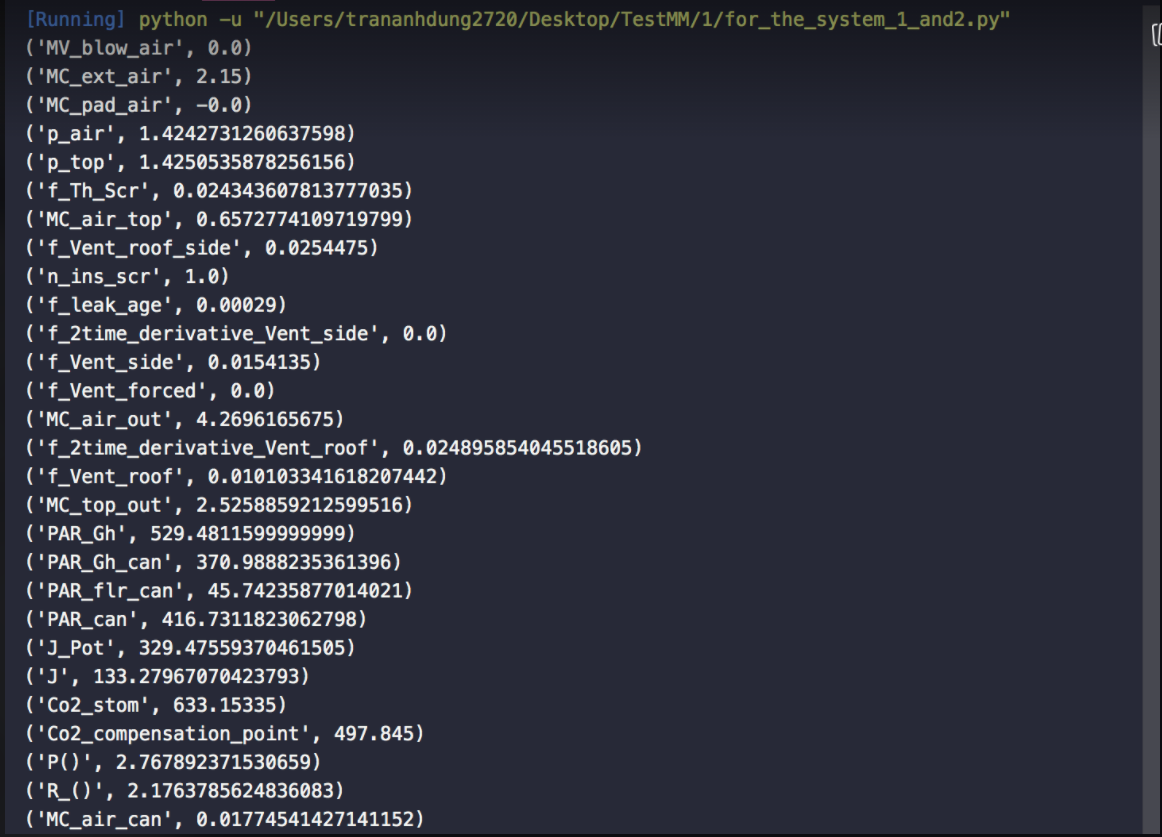
\includegraphics[width=15cm]{Result3.png}
    \end{figure}
    \item[-] This function will return two results: \(\dot{CO_{2Air}} = 0.3956060694677419\) and \(\dot{CO_{2Top}} = -18.176517952112416.\)\\
    This conclude that the CO2 concentration in the greenhouse air is slightly increase and CO2 concentration in the greenhouse air above the thermal screen is decrease at the summer time from day 157th to 162th.
\end{itemize}

	
\section{Calculating \texorpdfstring{\(CO_2\)}{} concentration with Euler and Runge-Kutta algorithms}
\subsection{Euler and Runge-Kutta of order 4 algorithms with python language}


\begin{itemize}
    \item Euler algorithm:
\end{itemize}

\begin{mdframed}[leftline=false,rightline=false,backgroundcolor=cyan!10,nobreak=false]
  \begin{minted}[linenos,breaklines,breaksymbolleft=,obeytabs=true,tabsize=2]{Python}
@dataclass
class Euler:
    x_0: float = 0.0
    y_0: float = 0.0
    t: float = 0.0
    h: float = 0.0

    def __init__(self, x0, y0, t0, h):
        self.x_0 = x0
        self.y_0 = y0
        self.t = t0
        self.h = h

    def calculateNewValue(self, x, y):
        x_new = x + self.dx_dt(x, y, self.t) * h
        y_new = y + self.dy_dt(x, y, self.t) * h

        return x_new, y_new

    def calculateNext(self, x, y):
        self.t = self.t + h

        yield self.calculateNewValue(x, y)

    def dx_dt(self, x, y, t):
        rhs = (
            MC_blow_air() + MC_ext_air()
            + ((U_pad * phi_pad)/A_flr) * (668.0 - x) #! MC_pad_out
            - f_Th_Scr() * (x - y) #! MC_air_top
            - (f_Vent_forced() + f_Vent_side()) #!MC_air_out
            - ((M_ch2o * J())/4.0) * ((n_Co2_air_stom * x - Co2_compensation_point()) / (n_Co2_air_stom * x + (2.0 * Co2_compensation_point()))) * (1 - (Co2_compensation_point() / (n_Co2_air_stom * x)))#!MC_air_can
        )
        return rhs / 4.7

    def dy_dt(self, x, y, t):
        rhs = (
            f_Th_Scr() * (x - y) #!MC_air_top
            - f_Vent_roof() * (y - 668) #!MC_top_out
        )
        return rhs / 0.4


print("RUNNING EULER")
x = 990.005 #550
y = 981.005 #545
t = 157.0
h = 0.25
a = x/(0.0409*44.01)
b = y/(0.0409*44.01)
euler = Euler(x, y, t, h)  # x_0, y_0, t_0, h

list_x = [x]
list_y = [y]
list_t = [t]
list_a = [a]
list_b = [b]
 
for n in range(20):
    t = t + h
    gen_new_val = euler.calculateNext(x, y)
    x, y = next(gen_new_val)
    a = x/(0.0409*44.01)
    b = y/(0.0409*44.01)
    if n < 5:
        print(f"step: {n + 1}")
        print(f"new x: {a}\nnew y: {b}\n\n")
    if n == 0 or n == 4 or n == 9 or n == 14 or n == 19:
        list_x.append(x)
        list_y.append(y)
        list_a.append(a)
        list_b.append(b)
        list_t.append(t)

plt.plot(list_t, list_a, "-b", label = "CO2_air")
plt.plot(list_t, list_b, "-r", label = "CO2_top")
plt.title("The CO2 concentration below and above the thermal screen from DOY 157-162")
plt.xlabel("time(days)")
plt.ylabel("CO2_concentration")
plt.legend()
#plt.subplot(1,1,1)
#plt.title("The CO2 concentration above the thermal screen from DOY 157-162")
#plt.xlabel("time(days)")
#plt.ylabel("CO2_top")

plt.show()
\end{minted}
\end{mdframed}



\begin{itemize}
    \item Runge-Kutta of order 4 algorithm:
\end{itemize}
\begin{mdframed}[leftline=false,rightline=false,backgroundcolor=cyan!10,nobreak=false]
  \begin{minted}[linenos,breaklines,breaksymbolleft=,obeytabs=true,tabsize=2]{Python}
# in the program, the function is named 'runge_kutta4th'
@dataclass
class RK4:
    x_0: float = 0.0
    y_0: float = 0.0
    t: float = 0.0
    h: float = 0.0

    def __init__(self, x0, y0, t0, h):
        self.x_0 = x0
        self.y_0 = y0
        self.t = t0
        self.h = h

    def calculateNewValue(self, x, y):
        k0_x, k0_y = self.calculateFirstSlop(x, y)
        k1_x, k1_y = self.calculateMiddleSlop(x, y, k0_x, k0_y)
        k2_x, k2_y = self.calculateMiddleSlop(x, y, k1_x, k1_y)
        k3_x, k3_y = self.calculateLastSlop(x, y, k2_x, k2_y)

        x_new = x + (k0_x + 2 * k1_x + 2 * k2_x + k3_x) / 6.0
        y_new = y + (k0_y + 2 * k1_y + 2 * k2_y + k3_y) / 6.0

        return x_new, y_new

    def calculateFirstSlop(self, x, y):
        k0_x = h * self.dx_dt(x, y, self.t)
        k0_y = h * self.dy_dt(x, y, self.t)

        return k0_x, k0_y

    def calculateMiddleSlop(self, x, y, k_prev_x, k_prev_y):
        k_next_x = h * self.dx_dt(
            x + k_prev_x * 0.5, y + k_prev_y * 0.5, self.t + h * 0.5
        )
        k_next_y = h * self.dy_dt(
            x + k_prev_x * 0.5, y + k_prev_y * 0.5, self.t + h * 0.5
        )

        return k_next_x, k_next_y

    def calculateLastSlop(self, x, y, k_prev_x, k_prev_y):
        k_last_x = h * self.dx_dt(x + k_prev_x, y + k_prev_y, self.t + h)
        k_last_y = h * self.dy_dt(x + k_prev_x, y + k_prev_y, self.t + h)

        return k_last_x, k_last_y

    def calculateNext(self, x, y):
        self.t = self.t + h

        yield self.calculateNewValue(x, y)

    def dx_dt(self, x, y, t):
        rhs = (
            MC_blow_air() + MC_ext_air()
            + ((U_pad * phi_pad)/A_flr) * (668.0 - x) #! MC_pad_out
            - f_Th_Scr() * (x - y) #! MC_air_top
            - (f_Vent_forced() + f_Vent_side()) #!MC_air_out
            - ((M_ch2o * J())/4.0) * ((n_Co2_air_stom * x - Co2_compensation_point()) / (n_Co2_air_stom * x + (2.0 * Co2_compensation_point()))) * (1 - (Co2_compensation_point() / (n_Co2_air_stom * x)))#!MC_air_can
        )
        return rhs / 4.7

    def dy_dt(self, x, y, t):
        rhs = (
            f_Th_Scr() * (x - y) #!MC_air_top
            - f_Vent_roof() * (y - 668) #!MC_top_out
        )
        return rhs / 0.4


print("RUNNING RK4")
x = 990.005 #550
y = 981.005 #545
t = 157.0
h = 0.25
a = x/(0.0409*44.01)
b = y/(0.0409*44.01)
rk4 = RK4(x, y, t, h)  # x_0, y_0, t_0, h

list_x = [x]
list_y = [y]
list_t = [t]
list_a = [a]
list_b = [b]

for n in range(20):
    t = t + h
    gen_new_val = rk4.calculateNext(x, y)
    x, y = next(gen_new_val)
    a = x/(0.0409*44.01)
    b = y/(0.0409*44.01)
    if n < 5:
        print(f"step: {n + 1}")
        print(f"new x: {a}\nnew y: {b}\n\n")
    if n == 0 or n == 4 or n == 9 or n == 14 or n == 19:   
        list_x.append(x)
        list_y.append(y)
        list_a.append(a)
        list_b.append(b)
        list_t.append(t)


#plt.subplot(1,1,1)
plt.plot(list_t, list_a, "-b", label = "CO2_air")
plt.plot(list_t, list_b, "-r", label = "CO2_top")
plt.title("The CO2 concentration below and above the thermal screen from DOY 157-162")
plt.xlabel("time(days)")
plt.ylabel("CO2_concentration")
plt.legend()
#plt.subplot(1,1,1)
#plt.title("The CO2 concentration above the thermal screen from DOY 157-162")
#plt.xlabel("time(days)")
#plt.ylabel("CO2_top")

plt.show()
  \end{minted}
\end{mdframed}

\subsection{Comparing to actual data and comment on accuracy of the model}
From initial state at which \(t_{0} = 157\), choosing \(CO_{2Air} = 990.005~mg m^{-3}  (= 550~ ppm)\) and \(CO_{2Top} = 981.005 ~ mg m^{-3} (=545~ppm)\) as initial values, we have the following approximation values of \(CO_{2Air}, CO_{2Top}\) in the next 5 minutes, 10 minutes, 20 minutes, 25 minutes, represented as the table below. The actual values of \(CO_{2Top}\) are not available for comparison.

\begin{itemize}
    \item The result of the program: x is $CO_{2Air}$ and y is $CO_{2Top}$
\end{itemize}

\begin{figure}[H]
  \centering
  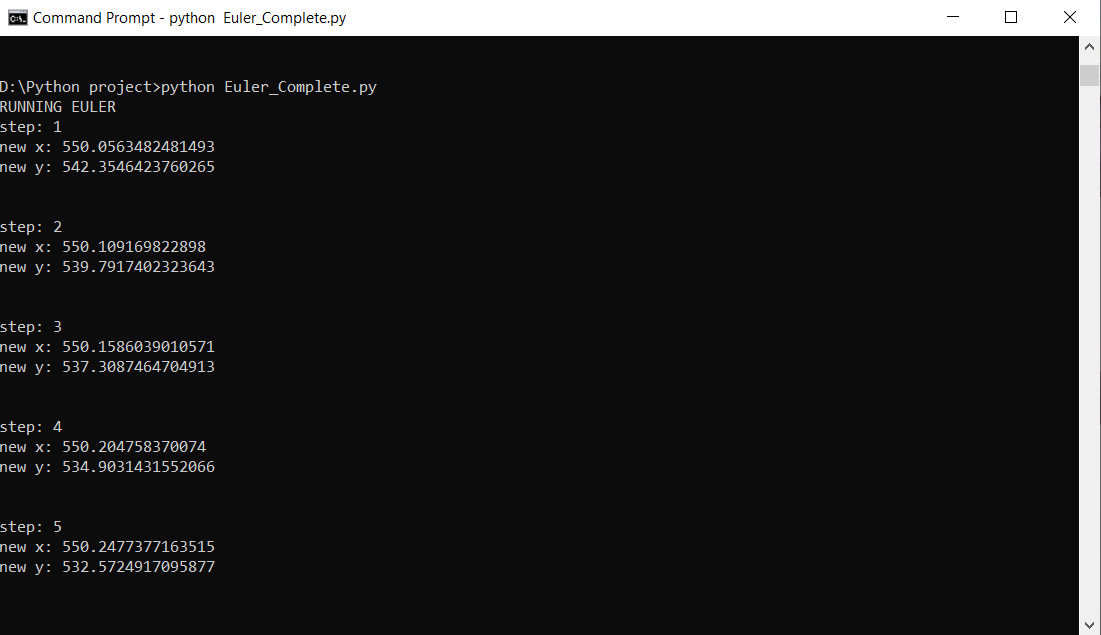
\includegraphics[width=15cm]{Result3_Euler.png}
\end{figure}
\begin{figure}[H]
  \centering
  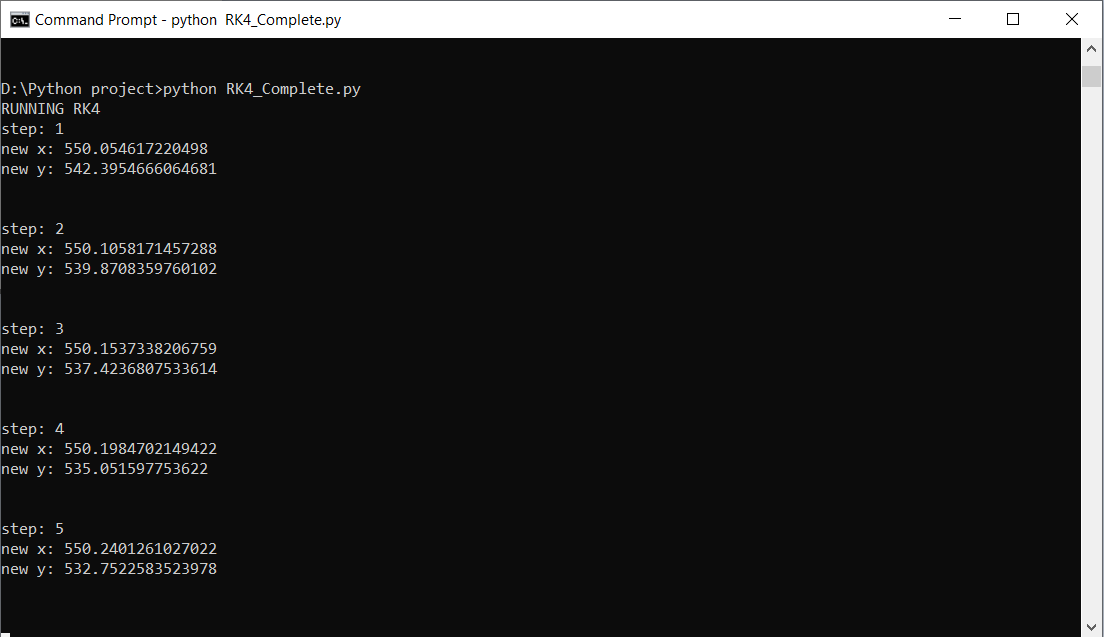
\includegraphics[width=15cm]{Result3_RK4.png}
\end{figure}

\begin{table}[H]
\begin{tabular}{lccccc}
\hline
\textbf{Time} & \multicolumn{1}{l}{\(CO_{2Air}\)(Euler)} & \multicolumn{1}{l}{\(CO_{2Air}\)(RK4)} & \multicolumn{1}{l}{\textbf{Actual data}} & \multicolumn{1}{l}{\textbf{Diff(Euler)}} & \multicolumn{1}{l}{\textbf{Diff(RK4)}} \\ \hline
5             & 550.0563                                 & 550.0546                               & 550.0500                                 & 0.0063                                   & 0.0046                                 \\
10            & 550.1092                                 & 550.1058                               & 550.1000                                 & 0.0092                                   & 0.0058                                 \\
15            & 550.1586                                 & 550.1537                               & 550.1300                                 & 0.0286                                   & 0.0237                                 \\
20            & 550.2048                                 & 550.1985                               & 550.1600                                 & 0.0448                                   & 0.0385                                 \\
25            & 550.2477                                 & 550.2401                               & 550.2000                                 & 0.0477                                   & 0.0401                                 \\ \hline
\end{tabular}
\end{table}

\begin{table}[H]
\begin{tabular}{lccccc}
\hline
\textbf{Time} & \multicolumn{1}{l}{\(CO_{2Top}\)(Euler)} & \multicolumn{1}{l}{\(CO_{2Top}\)(RK4)} & \multicolumn{1}{l}{\textbf{Actual data}} & \multicolumn{1}{l}{\textbf{Diff(euler)}} & \multicolumn{1}{l}{\textbf{Diff(rk4)}} \\ \hline
5             & 542.3546                                 & 542.3955                               & x                                        & x                                        & x                                      \\
10            & 539.7917                                 & 539.8708                               & x                                        & x                                        & x                                      \\
15            & 537.3087                                 & 537.4237                               & x                                        & x                                        & x                                      \\
20            & 534.9031                                 & 535.0516                               & x                                        & x                                        & x                                      \\
25            & 532.5725                                 & 532.7523                               & x                                        & x                                        & x                                      \\ \hline
\end{tabular}
\end{table}

\begin{itemize}
    \item The graph below is used to compare to actual data from Van11, the unit of $CO_{2}$ is changed to ppm to be similar to the references
\end{itemize}

\begin{figure}[H]
  \centering
  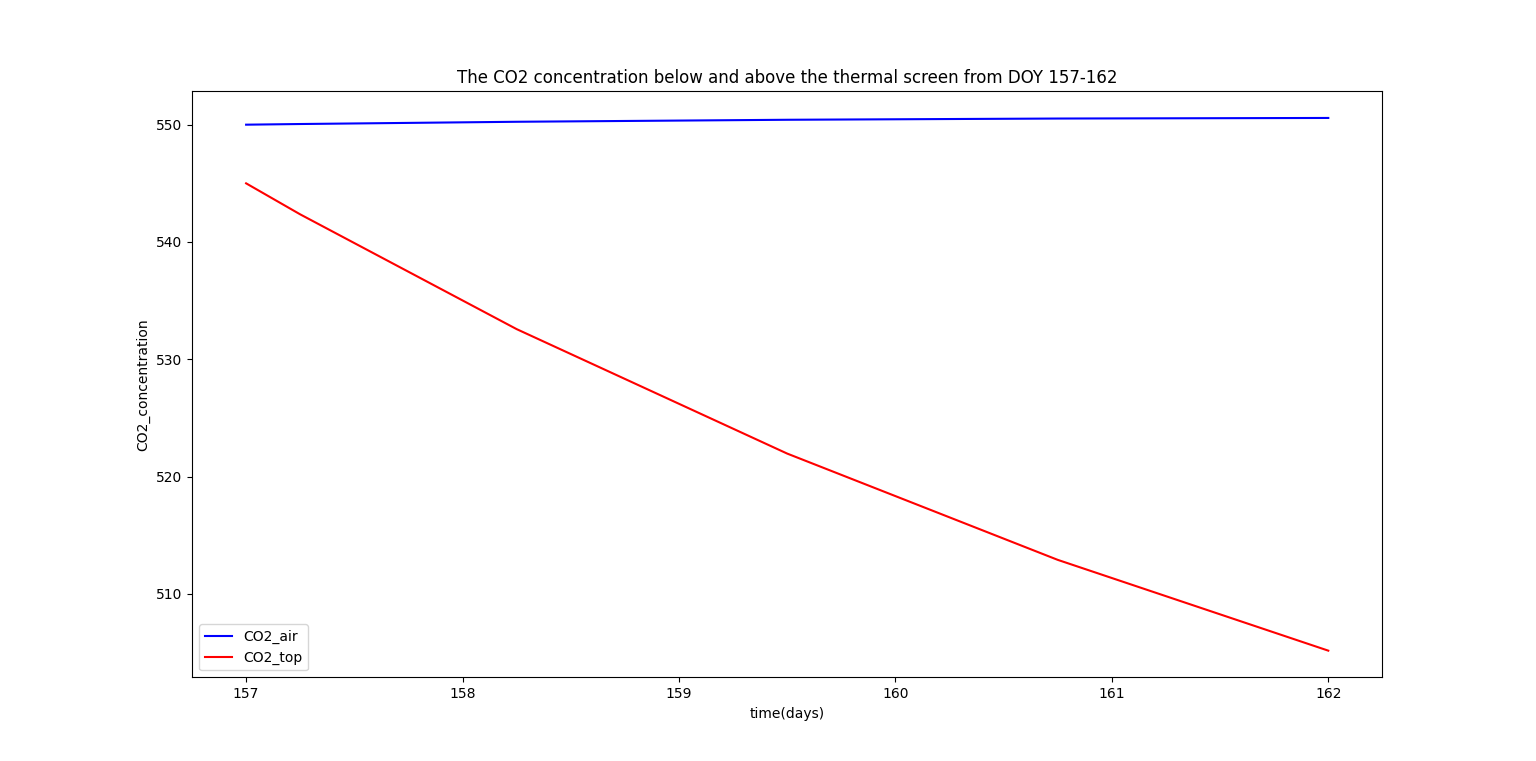
\includegraphics[width=16cm]{CO2_compare_Euler.png}
  \caption{Result of Euler method}
\end{figure}

\begin{figure}[H]
  \centering
  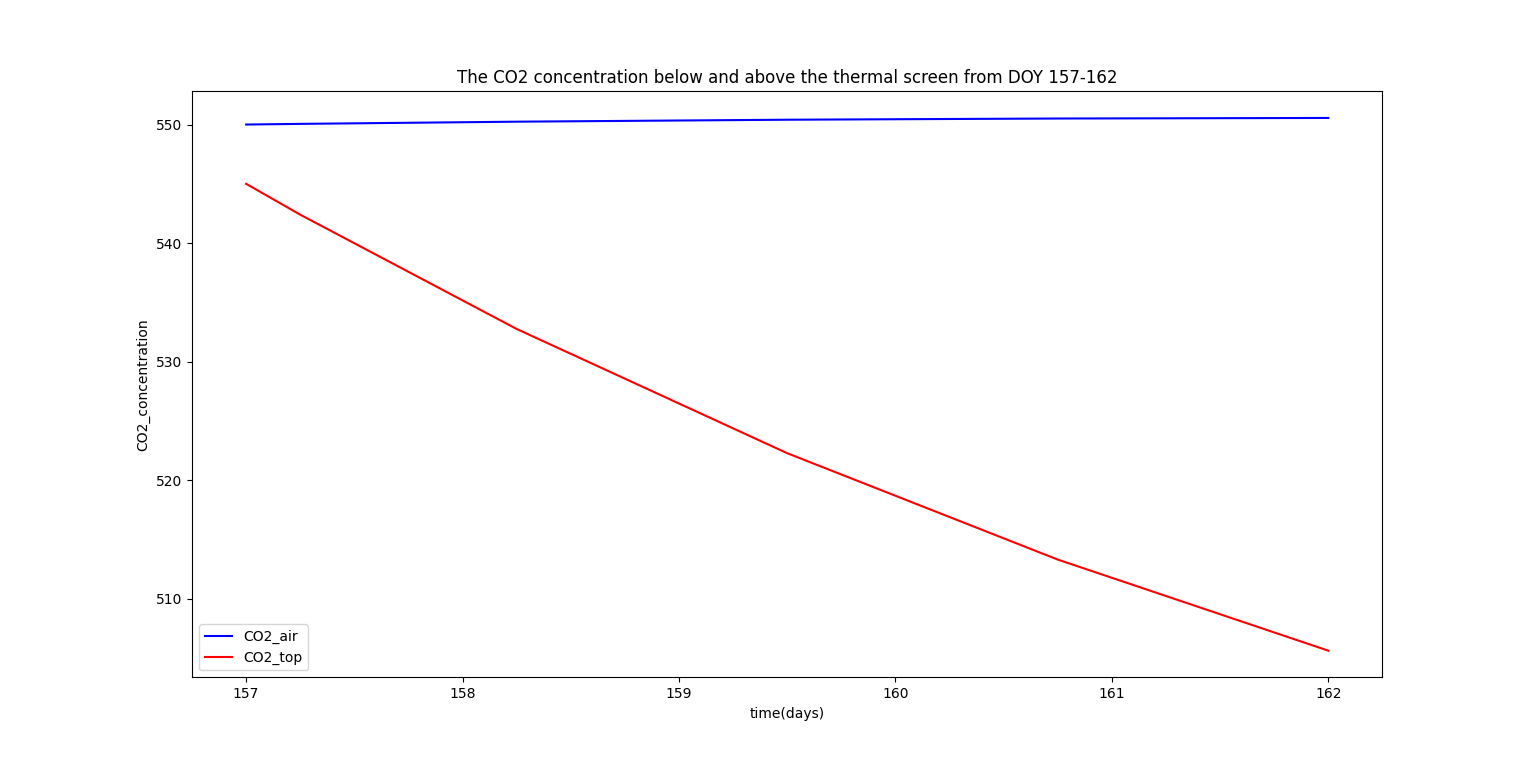
\includegraphics[width=16cm]{CO2_compare_RK4.png}
  \caption{Result of RK4 method}
\end{figure}

\begin{figure}[H]
  \centering
  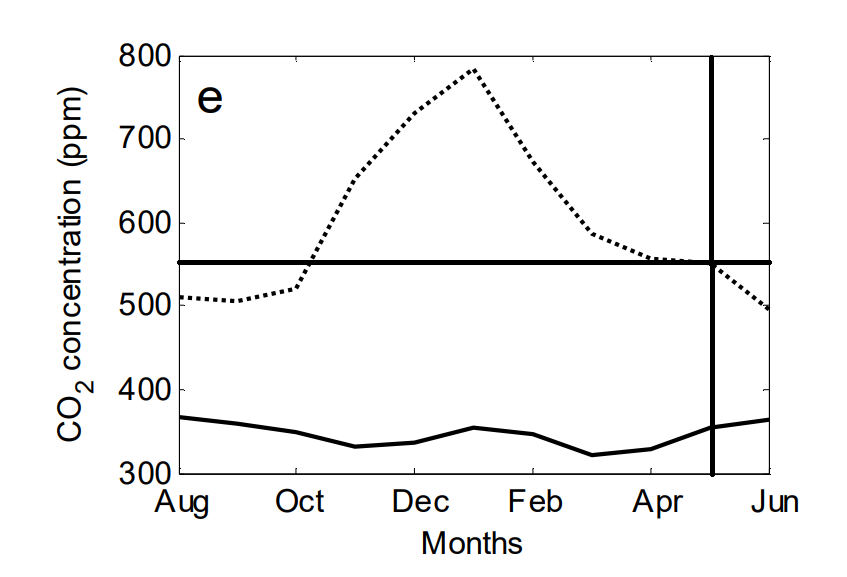
\includegraphics[width=12cm]{ActualData.png}
  \caption{Actual Data from Van11 page 97}
\end{figure}

Conclusion, during the summer time between day 157th to 162th, the CO2 concentration in actual data was slightly changed and result on the program is nearly accurate.

%%%%%%%%%%%%%%%%%
\section{Vapor pressure in greenhouse model}
\subsection{Theory}
Beside $CO_2$ concentration, the vapour pressure is also a factor that affect to crop yield that we have to control and it can be predicted through the model.
The vapour pressure of the greenhouse air \(VP_{Air}\) is described by:
\begin{multline*}
  cap_{VP_{Air}}\dot{VP_{Air}} = MV_{CanAir} + MV_{PadAir} + MV_{FogAir} + MV_{BlowAir} \\
  - MV_{AirThScr} - MV_{AirTop} - MV_{AirOut} \\
  - MV_{AirOut\_Pad} - MV_{AirMech} ~~~~ [kg\;m^{-2}\;s^{-1}]
\end{multline*}
\begin{itemize}
    \item \(cap_{VP_{Air}}\):the capacity of the air to store water vapor.
    \item \(MP_{CanAir}\): the canopy
    \item \(MV_{PadAir}\): The outlet air of the pad
    \item \(MV_{FogAir}\): the fogging system.
    \item \(MV_{BlowAir}\): the direct air heater.
    \item \(MV_{AirThScr}\): the Thermal screen.
    \item \(MV_{AirTop}\): the top compartment air
    \item \(MV_{AirOut}\): the outdoor air.
    \item \(MV_{AirOut\_Pad}\): the air exchange caused by the pad and fan system.
    \item \(MV_{AirMech}\): the mechanical cooling system
\end{itemize}
The vapour pressure of the air in the top compartment \(VP_{Top}\) is described by: 
\begin{multline*}
  cap_{VP_{Top}}\dot{VP_{Top}} = MV_{AirTop} - MV_{TopCov,in} - MV_{TopOut} ~~~~~~~~ [kg\ m^{-2}\ s^{-1}]
\end{multline*}
\begin{itemize}
    \item \(cap_{VP_{Top}}\): the capacity of the top compartment to store water vapour.
    \item \(MV_{TopCov,in}\): the vapour exchange between the top compartment and the internal cover.
    \item \(MV_{TopOut}\): the vapour exchange between the top compartment and the outside air.
\end{itemize}
\begin{align*}
    cap_{VPair} = \frac{M_{water}.h_{air}}{R(T_{Air+273.15})} [kgm^3J^{-1}]
\end{align*} 
\begin{align*}
    cap_{VPtop} = \frac{M_{water}.h_{top}}{R(T_{Top+273.15})} [kgm^3J^{-1}]
\end{align*}
\begin{itemize}
    \item \(cap_{VPair}\): water vapour capacity of the air compartment.
    \item \(M_{water}\): the molar mass of water
    \item \(h_{air}\):  the height from the floor to the thermal screen.
    \item \(h_{top}\):  the height from the floor to the thermal screen.
    \item R: the molar gas constant.
\end{itemize}
The vapor pressure of the air in the top compartment \(VP_{Top}\) is described by:
\begin{multline*}
  cap_{VP_{Top}}\dot{VP_{Top}} = MV_{AirTop} - MV_{TopCov,in} - MV_{TopOut} ~~~~~~~~ [kg\;m^{-2}\;s^{-1}]
\end{multline*}
\begin{itemize}
    \item \(cap_{VP_{Top}}\): the capacity of the top compartment to store water vapour.
    \item \(MV_{TopCov,in}\): the vapor exchange between the top compartment and the internal cover layer.
    \item \(MV_{TopOut}\): the vapor exchange between the top compartment and the outside air
\end{itemize}
The canopy transpiration is described by:
\begin{align*}
  MV_{CanAir} = VEC_{CanAir}(VP_{Can} - VP_{Air})
\end{align*}
\begin{itemize}
    \item \(VEC_{CanAir}\): the vapor exchange coefficient between the canopy and air
    \item \(VP_{Can}\): the saturated vapour pressure at canopy temperature.
\end{itemize}
Based on Stanghellini (1987), the value of the vapor transfer coefficient of the canopy transpiration can be calculated by the equation below:
\begin{align*}
  VEC_{CanAir} = \frac{2 \rho_{Air} c_{p,Air}LAI}{\Delta H \gamma (r_b + r_s)}
\end{align*}
\begin{itemize}
    \item \(\rho_{Air}\): the density of the greenhouse air
    \item \(c_{p,Air}\): the specific heat capacity of the greenhouse air.
    \item \(LAI\): the leaf area index.
    \item \(\Delta H\): the latent heat of evaporation of water.
    \item \(\gamma\): the psychometric constant
    \item \(r_b\): is the boundary layer resistance of the canopy for vapor transport
    \item \(r_s\): the stomatal resistance of the canopy for vapor transport.
\end{itemize}

Arcording to \cite{stanghellini1987transpiration}
 The wind speed in the greenhouse and the temperature difference between the canopy and surrounding air are together affect the value of the boundary layer resistance for vapor transport.
The stomatal resistance of the canopy is described by the formula below:
\begin{align*}
  r_s = r_{s,\min} \cdot rf(R_{Can}) \cdot rf(CO_{2Air\_ppm}) \cdot rf(VP_{Can} - VP_{Air})
\end{align*}
\begin{itemize}
    \item \(r_{s,\min}\): the minimum canopy resistance
    \item \(rf\): the resistance factor for high radiation levels
    \item high \(CO_2\): levels and large vapor pressure differences.
\end{itemize}
The resistance factors are described according to Stangellini (1987):
\begin{equation*}
  \begin{split}
    rf(R_{Can}) & = \frac{R_{Can} + c_{evap1}}{R_{Can} + c_{evap2}} \\
    rf(CO_{2Air}) & = 1 + {c_{evap3} (\eta_{mg\_ppm} CO_{2Air} - 200)}^2 \\
    rf(VP_{Can} - VP_{Air}) & = 1 + {c_{evap4} (VP_{Can} - VP_{Air})}^2
  \end{split}
\end{equation*}
\begin{itemize}
    \item \(R_{Can}\): the global radiation above the canopy
    \item \(c_{evap1}\) (\(W\;m^{-2}\)), \(c_{evap2}\) (\(W\;m^{-2}\)), \(c_{evap3}\) (\(ppm^{-2}\)), \(c_{evap4}\) (\(Pa^{-2}\)) are empirically determined parameters
    \item \(\eta_{mg\_ppm}\) (\(ppm\;mg^{-1}\;m^3\)) is the conversion factor from \(mg\;m^{-3}\;CO_2\) to \(ppm\)\\\\
    Stanghellini limited the resistance factor for high \(CO_2\) levels to 1.5 and the resistance factor for large vapor pressure differences to 5.8
    \item \(c_{evap3}\): the transpiration variables
    \item \(c_{evap4}\) for day time and night time.
\end{itemize}
The values of the transpiration parameters \(c_{evap3}\) and \(c_{evap4}\) differed between the night period and day period which means that the accompanying equations are not differentiable at sunrise and sunset. Therefore the parameters \(c_{evap3}\) and \(c_{evap4}\) were smoothed using the differentiable switch function:
\begin{align*}
  S_{r_s} = \frac{1}{1 + \exp \left(s_{r_s} (R_{Can} - R_{Can\_SP})\right)}
\end{align*}
\begin{itemize}
    \item \(S_{r_s}\): the value of the differentiable switch 
\end{itemize}
The vapor flux from the pad and fan to the greenhouse air is described by:
\begin{align*}
  MV_{PadAir} = \rho_{Air} f_{Pad} (\eta_{Pad} (x_{Pad} - x_{Out}) + x_{Out})
\end{align*}
\begin{itemize}
    \item \(f_{Pad}\): the ventilation flux due to the pad and fan system
    \item \(\eta_{Pad}\): the efficiency of the pad and fan system
    \item \(x_{Pad}\): the water vapor content of the pad
    \item \(x_{Out}\): the water vapor content of the outdoor air.
\end{itemize}
The latent heat flux from the greenhouse air depends on the vapor flux from the fogging system to the greenhouse air which is described by:
\begin{align*}
  MV_{FogAir} = \frac{U_{Fog} \phi_{Fog}}{A_{Flr}}
\end{align*}
\begin{itemize}
\item \(U_{Fog}\): the control valve of the fogging system
\item \(\phi_{Fog}\): the capacity of the fogging system.
\end{itemize}
The vapor flux from the heat blower to the greenhouse air is proportional to the heat flux:
\begin{align*}
  MV_{BlowAir} = \eta_{HeatVap} H_{BlowAir}
\end{align*}
\begin{itemize}
    \item \(\eta_{HeatVap}\): the amount of vapor which is released when 1 Joule of sensible energy is produced by the direct air heater..
\end{itemize}
The vapor exchange coefficient between the air and an object is linearly related to the convective heat exchange coefficient between the air and the object.
Therefore, the vapor flux from the air to an object by condensation is described by:
\begin{align*}
  \label{eq:vapor_conden}
  MV_{12} = \begin{cases}
    0                                       & \text{if~} VP_1 < VP_2 \\
    6.4 \cdot 10^{-9} HEC_{12}(VP_1 - VP_2) & \text{if~} VP_1 > VP_2 \\
  \end{cases}
\end{align*}
\begin{itemize}
    \item \(MV_{12}\): the vapor flux from air of location 1 to object 2.
    \item \(6.4 \cdot 10^{-9}\) is the conversion factor relating the heat exchange coefficient (\(W\;m^{-2}\;K^{-1}\)) to the vapor exchange coefficient (\(kg\;m^{-2}\;s^{-1}\;Pa^{-1}\)), \(HEC_{12}\) (\(W\;m^{-2}\;K^{-1}\)) is the heat exchange coefficient between the air of location 1 to object 2 and \(VP_1\) (\(Pa\)) is the vapor pressure of the air of location 1 and \(VP_2\) is the saturated vapor pressure of object 2 at its temperature.
\end{itemize}
The vapor flux from the greenhouse air compartment to the thermal screen and the vapor flux from the top compartment to the interval cover layer are described:
\begin{align*}
  MV_{AirThScr}  & = \begin{cases}
    0                                                       & \text{if~} VP_{Air} < VP_{ThScr} \\
    6.4 \cdot 10^{-9} HEC_{AirThScr}(VP_{Air} - VP_{ThScr}) & \text{if~} VP_{Air} > VP_{ThScr} \\
  \end{cases} \\
  % TopCov,in
  MV_{TopCov,in} & = \begin{cases}
    0                                                         & \text{if~} VP_{Top} < VP_{Cov,in} \\
    6.4 \cdot 10^{-9} HEC_{TopCov,in}(VP_{Top} - VP_{Cov,in}) & \text{if~} VP_{Top} > VP_{Cov,in} \\
  \end{cases}
\end{align*}
whereby their associated heat change coefficients are:
\begin{align*}
  HEC_{AirThScr}  & = 1.7 U_{ThScr} |T_{Air} - T_{ThScr}|^{0.33}                        \\
  HEC_{TopCov,in} & = {c_{HECin} (T_{Top} - T_{Cov,in})}^{0.33} \frac{A_{Cov}}{A_{Flr}}
\end{align*}\\
\begin{itemize}
    \item \(U_{ThScr} \in [0,1]\) representing the percentage of places that are covered by the thermal screen.
    \item \(T_X\) (\(\celsius\)) is the temperature at location.
    \item \(X\), \(c_{HECin}\): the convective heat exchange parameter between cover and outdoor air depending on the greenhouse shape.
    \item \(A_{Cov}\): the surface of the cover including the side-walls.
    \item \(A_{Flr}\): the surface of the greenhouse floor.
\end{itemize}
The vapor flux from the greenhouse air to the outside air when using the pad and fan system is described by:
\begin{align*}
  MV_{AirOut\_Pad} = f_{Pad} \frac{M_{Water}}{R} \left(\frac{VP_{Air}}{T_{Air} + 273.15}\right)
\end{align*}

% AirMech
The vapor flux from the greenhouse air to the surface of mechanical cooling system.
\begin{align*}
  MV_{AirMech} = \begin{cases}
    0                                                     & \text{if~} VP_{Air} < VP_{Mech} \\
    6.4 \cdot 10^{-9} HEC_{AirMech}(VP_{Air} - VP_{Mech}) & \text{if~} VP_{Air} > VP_{Mech} \\
  \end{cases}
\end{align*}
with \(HEC_{AirMech}\) is the heat exchange coefficient between the greenhouse air and the surface of the mechanical cooling unit:
\begin{align*}
  HEC_{AirMech} = \frac{U_{MechCool} COP_{MechCool} P_{MechCool} / A_{Flr}}{T_{Air} - T_{MechCool} + 6.4 \cdot 10^{-9} \Delta H(VP_{Air} - VP_{MechCool})}
\end{align*}
\begin{itemize}
    \item \(U_{MechCool}\): the control valve of the mechanical cooling mechanism.
    \item \(COP_{MechCool}\): the coefficient of performance of the mechanical cooling system.
    \item \(P_{MechCool}\): the electrical capacity of the mechanical cooling system.
    \item \(T_{MechCool}\) (\(\celsius\)) is the temperature of the cooling surface.
    \item \(VP_{MechCool}\) (\(Pa\)) is the saturated vapor pressure of the mechanical cooling mechanism.
\end{itemize}
\subsection{Implement the program}

\begin{itemize}
    \item   $cap_{VPair} = \frac{M_{water}.h_{air}}{R(T_{Air+273.15})} ~~[kgm^3J^{-1}]$
\end{itemize}


\begin{mdframed}[leftline=false,rightline=false,backgroundcolor=cyan!10]
  \begin{minted}[linenos,breaklines,breaksymbolleft=,obeytabs=true,tabsize=2]{Python}
def cap_Vp_air(): #* equation 8.25
    return (M_water * h_air)/(R * (T_air + 273.15))
print("cap_Vp_air",cap_Vp_air())
\end{minted}
\end{mdframed}
\begin{table}[H]
\centering
\begin{tabular}{|l|l|l|l|}
\hline
\rowcolor[HTML]{FFFC9E} 
\textbf{$M_{water}$} & \textbf{$h_{air}$} & \cellcolor[HTML]{FFFC9E}\textbf{$R$} & \cellcolor[HTML]{FFFC9E}\textbf{$T_{Air}$}\\ \hline
18            &     4.7           &   $8.314*10^3$          &       291.15                \\ \hline
\end{tabular}
\end{table}
$\rightarrow cap_{VPAir} = 3.494970774*10^{-5}$
\begin{itemize}
    \item $cap_{VPtop} = \frac{M_{water}.h_{top}}{R(T_{Top+273.15})}      ~~[kgm^3J^{-1}] $
\end{itemize}

\begin{mdframed}[leftline=false,rightline=false,backgroundcolor=cyan!10]
  \begin{minted}[linenos,breaklines,breaksymbolleft=,obeytabs=true,tabsize=2]{Python}
def cap_Vp_top(): #* equation 8.25
    return (M_water * h_top)/(R * (T_air + 273.15))
print("cap_Vp_top",cap_Vp_top())
\end{minted}
\end{mdframed}
\begin{table}[H]
\centering
\begin{tabular}{|l|l|l|l|}
\hline
\rowcolor[HTML]{FFFC9E} 
\textbf{$M_{water}$} & \textbf{$h_{top}$} & \cellcolor[HTML]{FFFC9E}\textbf{$R$} & \cellcolor[HTML]{FFFC9E}\textbf{$T_{Top}$}\\ \hline
18            &     0.4           &   $8.314*10^3$          &       295.15                \\ \hline
\end{tabular}
\end{table}
$\rightarrow cap_{VpTop} = 2.934132279*10^{-6}$
\begin{itemize}
    \item $ S_{r_s} = \frac{1}{1 + \exp \left(s_{r_s} (R_{Can} - R_{Can\_SP})\right)}$
\end{itemize}


\begin{mdframed}[leftline=false,rightline=false,backgroundcolor=cyan!10]
  \begin{minted}[linenos,breaklines,breaksymbolleft=,obeytabs=true,tabsize=2]{Python}
def S_r_s(): #* equation 8.51 (maybe this equation is redundant)
    return 1.0/(1.0 + math.exp(s_r_s * (R_can - R_can_sp)))
print("S_r_s",S_r_s())
\end{minted}
\end{mdframed}

The value of $R_{can}$ is collected from the research of Michael E.Webber: "The Energy-Water Nexus: Spatially-Resolved Analysis of the Potential for Desalinating Brackish Groundwater by Use of Solar Energy" June 2015.

\begin{table}[H]
\centering
\begin{tabular}{|l|l|l|}
\hline
\rowcolor[HTML]{FFFC9E} 
\textbf{$s_{r_s}$} & \textbf{$R_{can}$} & \cellcolor[HTML]{FFFC9E}\textbf{$R_{can_{sp}}$} \\ \hline
-1.0           & 0.5439815        & 5.0                    \\ \hline
\end{tabular}
\end{table}
\begin{itemize}
    \item $c_{evap3} = c_{evap3}^{night} (1 - S_{r_s}) + c_{evap3}^{night} S_{r_s} $\\
    \item $c_{evap4} = c_{evap4}^{night} (1 - S_{r_s}) + c_{evap4}^{night} S_{r_s}$
\end{itemize}

\begin{mdframed}[leftline=false,rightline=false,backgroundcolor=cyan!10]
  \begin{minted}[linenos,breaklines,breaksymbolleft=,obeytabs=true,tabsize=2]{Python}
def c_evap_3(): #* equation 8.52
    return c_evap_night_3 #! explain in detail in report
print("c_evap_3",c_evap_3())
def c_evap_4(): #* equation 8.52
    return c_evap_day_4 #! read van11 on page 218
print("c_evap_4",c_evap_4())
\end{minted}
\end{mdframed}
\begin{table}[H]
\centering
\begin{tabular}{|l|l|}
\hline
\rowcolor[HTML]{FFFC9E} 
\textbf{$e^{night}_{evap3}$} & \textbf{$e^{night}_{evap4}$}  \\ \hline
$1.1*10^{-11}$           & $5.2*10^{-6}$                                 \\ \hline
\end{tabular}
\end{table}
\begin{itemize}
    \item $ rf(R_{Can}) = \frac{R_{Can} + c_{evap1}}{R_{Can} + c_{evap2}} $ \\
    \item $ rf(CO_{2Air}) = 1 + {c_{evap3} (\eta_{mg\_ppm} CO_{2Air} - 200)}^2$  \\
    \item $ rf(VP_{Can} - VP_{Air}) = 1 + {c_{evap4} (VP_{Can} - VP_{Air})}^2 $ \\
\end{itemize}

\begin{mdframed}[leftline=false,rightline=false,backgroundcolor=cyan!10]
  \begin{minted}[linenos,breaklines,breaksymbolleft=,obeytabs=true,tabsize=2]{Python}
def rf_R_can(): #* equation 8.50
    return (R_can + c_evap_1)/(R_can + c_evap_2)
print("rf_R_can",rf_R_can())
def rf_Co2_air(): #* equation 8.50
    return 1.0 + c_evap_3() * ((n_mg_ppm * Co2_air - 200.0) ** 2.0)
print("rf_Co2_air",rf_Co2_air())
def rf_Vpcan_Vpair(): #* equation 8.50
    return 1.0 + c_evap_4() * ((Vp_can - Vp_air) ** 2.0)
print("rf_Vpcan_Vpair",rf_Vpcan_Vpair())
\end{minted}
\end{mdframed}

\begin{table}[H]
\centering
\begin{tabular}{|l|l|}
\hline
\rowcolor[HTML]{FFFC9E} 
\textbf{$c_{evap1}$} & \textbf{$c_{evap2}$}  \\ \hline
  4.3        &    0.54                             \\ \hline
\end{tabular}
\end{table}

The value of $CO2_{Air}$ is the initial value of $CO2_{Air}$ which is assumed in question 3

\begin{table}[H]
\centering
\begin{tabular}{|l|l|l|}
\hline
\rowcolor[HTML]{FFFC9E} 
\textbf{$c_{evap3}$} & \textbf{$\eta_{mg\_ppm}$} & \cellcolor[HTML]{FFFC9E}\textbf{$CO_{2Air}$}\\ \hline
$1.1*10^{-11}$            &  0.554              &  990.005                 \\ \hline
\end{tabular}
\end{table}

*All the data collected in Van11's book (1991) are precise in times from day 157th to 162th. So the initial value of $VP_{air}$, $VP_{top}$ and the value of $VP_{can}$ is assumed based on the figure below from Van11 (page 40):
\begin{figure}[H]
    \centering
    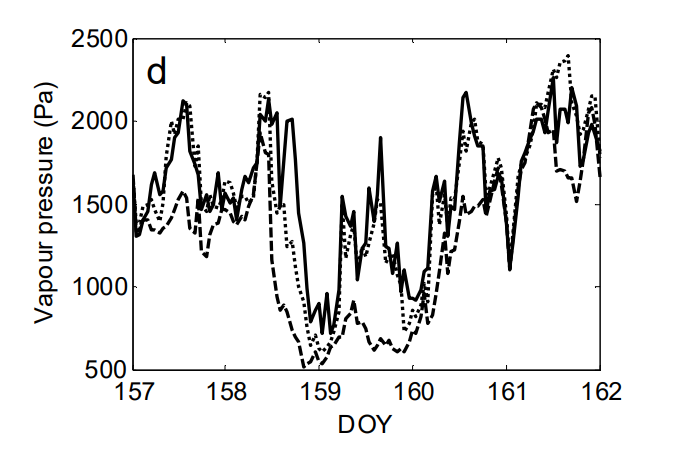
\includegraphics[width=0.75\textwidth]{VP.png}
\end{figure}

\begin{table}[H]
\centering
\begin{tabular}{|l|l|l|}
\hline
\rowcolor[HTML]{FFFC9E} 
\textbf{$c_{evap4}$} & \textbf{$VP_{Can}$} & \cellcolor[HTML]{FFFC9E}\textbf{$VP_{Air}$}\\ \hline
$5.2*10^{-6}$             &  2300              &  1700               \\ \hline
\end{tabular}
\end{table}


\begin{itemize}
    \item $ r_s = r_{s,\min} \cdot rf(R_{Can}) \cdot rf(CO_{2Air\_ppm}) \cdot rf(VP_{Can} - VP_{Air})$
\end{itemize}
\begin{mdframed}[leftline=false,rightline=false,backgroundcolor=cyan!10]
  \begin{minted}[linenos,breaklines,breaksymbolleft=,obeytabs=true,tabsize=2]{Python}
def r_s(): #* equation 8.49
    return r_s_min * rf_R_can() * rf_Co2_air() * rf_Vpcan_Vpair()
print("r_s",r_s())
\end{minted}
\end{mdframed}
\begin{table}[H]
\centering
\begin{tabular}{|l|l|l|l|}
\hline 
\rowcolor[HTML]{FFFC9E} 
\textbf{$r_{smin}$} & \textbf{$rf_{Rcan}$} & \cellcolor[HTML]{FFFC9E}\textbf{$rf_{CO2Air}$} & \cellcolor[HTML]{FFFC9E}\textbf{$rf_{VpcanVpair}$}\\ \hline
82            &  2.4434182609901476               & 1.0000011514079858            &  2.872                      \\ \hline
\end{tabular}
\end{table}
$\rightarrow r_{s} = 575.4354366964179$

\begin{itemize}
    \item $ VEC_{CanAir} = \frac{2 \rho_{Air} c_{p,Air}LAI}{\Delta H \gamma (r_b + r_s)}$
\end{itemize}
\begin{mdframed}[leftline=false,rightline=false,backgroundcolor=cyan!10]
  \begin{minted}[linenos,breaklines,breaksymbolleft=,obeytabs=true,tabsize=2]{Python}
def VEC_can_air(): #* equation 8.48
    return (2.0 * p_air() * c_p_air * L_a_i)/(delta_H * gamma * (r_b + r_s()))
print("VEC_can_air",VEC_can_air())
\end{minted}
\end{mdframed}

The value of $p_{air}$ is already calculated in question 3, so we reused it

\begin{table}[H]
\centering
\begin{tabular}{|l|l|l|l|l|l|l|}
\hline
\rowcolor[HTML]{FFFC9E} 
\textbf{$p_{air}$} & \textbf{$c_{pair}$} & \cellcolor[HTML]{FFFC9E}\textbf{$LAI$} & \cellcolor[HTML]{FFFC9E}\textbf{$\delta H$}& \cellcolor[HTML]{FFFC9E}\textbf{$\gamma$}& \cellcolor[HTML]{FFFC9E}\textbf{$r_b$}& \cellcolor[HTML]{FFFC9E}\textbf{$r_s$}\\ \hline
1.4242731260637596            &$10^{3}$                & 2.0            & $2.45*10^{6}$     &65.8  &275  &  575.4354366964179               \\ \hline
\end{tabular}
\end{table}
$\rightarrow VEC_{CanAir} = 4.1554680236317574*10^{-08}$

\begin{itemize}
    \item $ MV_{CanAir} = VEC_{CanAir}(VP_{Can} - VP_{Air})$
\end{itemize}
\begin{mdframed}[leftline=false,rightline=false,backgroundcolor=cyan!10]
  \begin{minted}[linenos,breaklines,breaksymbolleft=,obeytabs=true,tabsize=2]{Python}
def MV_can_air(): #* equation 8.47
    return (VEC_can_air() * (Vp_can - Vp_air))
print("MV_can_air",MV_can_air())
\end{minted}
\end{mdframed}
\begin{table}[H]
\centering
\begin{tabular}{|l|l|l|}
\hline
\rowcolor[HTML]{FFFC9E} 
\textbf{$VEC_{canair}$} & \textbf{$VP_{can}$} & \cellcolor[HTML]{FFFC9E}\textbf{$VP_{air}$}\\ \hline
$4.1554680236317574*10^{-08}$            & 2300               &  1700                 \\ \hline
\end{tabular}
\end{table}
$\rightarrow MV_{CanAir} = 2.4932808141790545*10^{-5}$

\begin{itemize}
    \item $ MV_{BlowAir} = \eta_{HeatVap} H_{BlowAir}$
\end{itemize}
\begin{mdframed}[leftline=false,rightline=false,backgroundcolor=cyan!10]
  \begin{minted}[linenos,breaklines,breaksymbolleft=,obeytabs=true,tabsize=2]{Python}
def MV_blow_air(): #* equation 8.55
    return (n_heat_vap * U_blow * P_blow)/A_flr
print("MV_blow_air",MV_blow_air())
\end{minted}
\end{mdframed}
$H_{BlowAir} = \frac{U_{Blow}.P_{Blow}}{A_flr}$
Since $P_{Blow} = 0$, we get $H_{BlowAir}$
$\rightarrow MV_{BlowAir} = 0$

\begin{itemize}
    \item $ f_{Pad} = \frac{U_{Pad} \phi_{Pad}}{A_{Flr}}$
\end{itemize}
\begin{mdframed}[leftline=false,rightline=false,backgroundcolor=cyan!10]
  \begin{minted}[linenos,breaklines,breaksymbolleft=,obeytabs=true,tabsize=2]{Python}
def f_pad(): #* to help equation 8.58
    return (U_pad * phi_pad)/A_flr
print("f_pad",f_pad())
\end{minted}
\end{mdframed}
Since the greenhouse model in Texas does not have pad system, $\phi Pad = 0$, we get $f_{Pad} = 0$. So:

\begin{itemize}
    \item $ MV_{PadAir} = \rho_{Air} f_{Pad} (\eta_{Pad} (x_{Pad} - x_{Out}) + x_{Out}) = 0$
\end{itemize}
\begin{mdframed}[leftline=false,rightline=false,backgroundcolor=cyan!10]
  \begin{minted}[linenos,breaklines,breaksymbolleft=,obeytabs=true,tabsize=2]{Python}
def MV_pad_air(): #* equation 8.58
    return p_air() * f_pad() * (n_pad * (x_pad - x_out) + x_out)
print("MV_pad_air",MV_pad_air())
\end{minted}
\end{mdframed}

Similarity, we get the value of $MV_{AirOut\_Pad}$ equal to 0.
\begin{itemize}
    \item $ MV_{AirOut\_Pad} = f_{Pad} \frac{M_{Water}}{R} \left(\frac{VP_{Air}}{T_{Air} + 273.15}\right) = 0$
\end{itemize}
\begin{mdframed}[leftline=false,rightline=false,backgroundcolor=cyan!10]
  \begin{minted}[linenos,breaklines,breaksymbolleft=,obeytabs=true,tabsize=2]{Python}
def MV_air_out_pad(): #* equation 8.62
    return (f_pad() * M_water * Vp_air)/(R * (T_air + 273.15))
print("MV_air_out_pad",MV_air_out_pad())
\end{minted}
\end{mdframed}

Since the greenhouse model in Texas does not have fogging system pad, $\phi_{Fog}$ =  0, we get $f_{Fog} = 0$. 
\begin{itemize}
    \item $MV_{FogAir} = \frac{U_{Fog} \phi_{Fog}}{A_{Flr}} = 0$
\end{itemize}
\begin{mdframed}[leftline=false,rightline=false,backgroundcolor=cyan!10]
  \begin{minted}[linenos,breaklines,breaksymbolleft=,obeytabs=true,tabsize=2]{Python}
def MV_frog_air(): #* equation 8.64
    return (U_frog * phi_frog)/A_flr
print("MV_frog_air",MV_frog_air())
\end{minted}
\end{mdframed}

\begin{itemize}
    \item $MV_{AirTop} = \frac{M_{Water}}{R} f_{ThScr} \left(\frac{VP_{Air}}{T_{Air} + 273.15} - \frac{VP_{Top}}{T_{Top} + 273.15}\right)    $
\end{itemize}
\begin{mdframed}[leftline=false,rightline=false,backgroundcolor=cyan!10]
  \begin{minted}[linenos,breaklines,breaksymbolleft=,obeytabs=true,tabsize=2]{Python}
def MV_air_top(): #* equation 8.45 and according to van11 on page 216, f_air_top = f_Th_Scr 
    return (M_water/R) * f_Th_Scr() * (Vp_air/(T_air + 273.15) - Vp_top/(T_top + 273.15))
print("MV_air_top",MV_air_top())
\end{minted}
\end{mdframed}

The value of $f_{ThScr}$ is already calculated in question 3, so we reused it

\begin{table}[H]
\centering
\begin{tabular}{|l|l|l|l|l|l|l|}
\hline
\rowcolor[HTML]{FFFC9E} 
\textbf{$M_{water}$} & \textbf{$R$} & \cellcolor[HTML]{FFFC9E}\textbf{$f_{ThScr}$} & \cellcolor[HTML]{FFFC9E}\textbf{$VP_{Air}$}& \cellcolor[HTML]{FFFC9E}\textbf{$T_{Air}$}& \cellcolor[HTML]{FFFC9E}\textbf{$VP_{Top}$}& \cellcolor[HTML]{FFFC9E}\textbf{$T_{Top}$}\\ \hline
18            & 8314               &0.0243443             &1700      &291.15  & 1650 & 295.15                \\ \hline
\end{tabular}
\end{table}
$\rightarrow MV_{AirTop} = 1.3098215855448786*10^{-5}$


\begin{itemize}
    \item $MV_{AirOut} = \frac{M_{Water}}{R} (f_{VentSide} + f_{VentForced}) \left(\frac{VP_{Air}}{T_{Air} + 273.15} - \frac{VP_{Out}}{T_{Out} + 273.15}\right)   $
\end{itemize}
\begin{mdframed}[leftline=false,rightline=false,backgroundcolor=cyan!10]
  \begin{minted}[linenos,breaklines,breaksymbolleft=,obeytabs=true,tabsize=2]{Python}
def MV_air_out(): #* equation 8.45 and according to van11 on page 216, f_air_out = f_vent_side + f_vent_forced
    return (M_water/R) * (f_Vent_side() + f_Vent_forced()) * (Vp_air/(T_air + 273.15) - Vp_out/(T_out + 273.15))
print("MV_air_out",MV_air_out())
\end{minted}
\end{mdframed}

\begin{table}[H]
\centering
\begin{tabular}{|l|l|l|l|}
\hline 
\rowcolor[HTML]{FFFC9E} 
\textbf{$f_{VentSide}$} & \textbf{$f_{VentForced}$} & 
\cellcolor[HTML]{FFFC9E}\textbf{$VP_{Out}$} &
\cellcolor[HTML]{FFFC9E}\textbf{$T_{Out}$}\\ \hline
0.000145                      & 0           &1000   & 297.05                  \\ \hline
\end{tabular}
\end{table}
$\rightarrow MV_{AirOut} = 8.100860849924075*10^{-5}$


\begin{itemize}
    \item $ MV_{TopOut}  = \frac{M_{Water}}{R} f_{VentRoof} \left(\frac{VP_{Top}}{T_{Top} + 273.15} - \frac{VP_{Out}}{T_{Out} + 273.15}\right)   $
\end{itemize}
\begin{mdframed}[leftline=false,rightline=false,backgroundcolor=cyan!10]
  \begin{minted}[linenos,breaklines,breaksymbolleft=,obeytabs=true,tabsize=2]{Python}
def MV_top_out(): #* equation 8.45 and according to van11 on page 216, f_top_out = f_vent_roof
   return (M_water/R) * f_Vent_roof() * (Vp_top/(T_top + 273.15) - Vp_out/(T_out + 273.15))
print("MV_top_out",MV_top_out())
\end{minted}
\end{mdframed}
$f_{VentRoof} = f''_{VentRoof} + 0.5f_{leakage} = 0.023783370636791715 + 0.5*0.00029 = 0.02392837064$
$\rightarrow MV_{TopOut} = 4.766389152705058*10^{-5}$

\begin{itemize}
    \item $ HEC_{TopCov,in} = {c_{HECin} (T_{Top} - T_{Cov,in})}^{0.33} \frac{A_{Cov}}{A_{Flr}}$
    \item $ HEC_{AirThScr} = 1.7 U_{ThScr} |T_{Air} - T_{ThScr}|^{0.33}$
    \item $ HEC_{AirMech} = \frac{U_{MechCool} COP_{MechCool} P_{MechCool} / A_{Flr}}{T_{Air} - T_{MechCool} + 6.4 \cdot 10^{-9} \Delta H(VP_{Air} - VP_{MechCool})}  $
\end{itemize}
\begin{mdframed}[leftline=false,rightline=false,backgroundcolor=cyan!10]
  \begin{minted}[linenos,breaklines,breaksymbolleft=,obeytabs=true,tabsize=2]{Python}
def HEC_top_cov_in(): #* to cal MV_top_cov_in
    return (c_HEC_in * A_cov * ((T_top - T_cov_in) ** 0.33))/A_flr #! be careful of negative number power a float number
print("HEC_top_cov_in",HEC_top_cov_in())

def HEC_air_Th_Scr(): #* to cal MV_air_Th_Scr
    return 1.7 * U_Th_Scr * (abs(T_air - T_Th_Scr) ** 0.33)
print("HEC_air_Th_Scr",HEC_air_Th_Scr())

def HEC_air_mech():#*equation 8.63 to cal MV_air_mech
    numerator = (U_mech_cool * Cop_mech_cool * P_mech_cool)/A_flr
    denominator = T_air - T_mech_cool + 6.4 * (10.0 **(-9.0)) * delta_H * (Vp_air - Vp_mach_cool)
    return numerator/denominator
print("HEC_air_mech",HEC_air_mech())
\end{minted}
\end{mdframed}

\begin{table}[H]
\centering
\begin{tabular}{|l|l|l|l|l|}
\hline
\rowcolor[HTML]{FFFC9E}
\cellcolor[HTML]{FFFC9E}\textbf{$c_{HECin}$} &
\textbf{$T_{Top}$} & \textbf{$T_{Cov,in}$} &  \cellcolor[HTML]{FFFC9E}\textbf{$A_{Cov}$}& \cellcolor[HTML]{FFFC9E}\textbf{$A_{Flr}$}\\ \hline
1.86            & 295.15               &294.05             &90000      & 78000                \\ \hline
\end{tabular}
\end{table}
$\rightarrow HEC_{TopCov,in} = 2.2147282078336135$

\begin{table}[H]
\centering
\begin{tabular}{|l|l|l|}
\hline
\rowcolor[HTML]{FFFC9E}
\cellcolor[HTML]{FFFC9E}\textbf{$U_{ThScr}$} &
 \cellcolor[HTML]{FFFC9E}\textbf{$T_{Air}$}& \cellcolor[HTML]{FFFC9E}\textbf{$T_{ThScr}$}\\ \hline
0.4            & 291.15               &  294.05                        \\ \hline
\end{tabular}
\end{table}
$\rightarrow HEC_{AirThScr} = 0.966273906746953$

\begin{itemize}
    \item $ MV_{AirMech} = \begin{cases}
    0                                                     & \text{if~} VP_{Air} < VP_{Mech} \\
    6.4 \cdot 10^{-9} HEC_{AirMech}(VP_{Air} - VP_{Mech}) & \text{if~} VP_{Air} > VP_{Mech} \\
  \end{cases}  $
\end{itemize}
\begin{mdframed}[leftline=false,rightline=false,backgroundcolor=cyan!10]
  \begin{minted}[linenos,breaklines,breaksymbolleft=,obeytabs=true,tabsize=2]{Python}
Vp_mech = 0.0
def MV_air_mech(): #* equation 8.43 page 221
    if Vp_air <= Vp_mech :
        return 0
    else :
        return 6.4 * (10.0 ** (-9.0)) * HEC_air_mech() * (Vp_air - Vp_mech)
print("MV_air_mech",MV_air_mech())
\end{minted}
\end{mdframed}
Since the greenhouse model in Texas does not have cooling system, we get $MV_{AirMech} = 0$.

\begin{itemize}
    \item $  MV_{AirThScr}   = \begin{cases}
    0                                                       & \text{if~} VP_{Air} < VP_{ThScr} \\
    6.4 \cdot 10^{-9} HEC_{AirThScr}(VP_{Air} - VP_{ThScr}) & \text{if~} VP_{Air} > VP_{ThScr} \\
  \end{cases}  $
\end{itemize}
\begin{mdframed}[leftline=false,rightline=false,backgroundcolor=cyan!10]
  \begin{minted}[linenos,breaklines,breaksymbolleft=,obeytabs=true,tabsize=2]{Python}
Vp_Th_Scr = 0.0
def MV_air_Th_Scr(): #* equation 8.43 page 215
    if Vp_air <= Vp_Th_Scr :
        return 0
    else :
        return 6.4 * (10.0 ** (-9.0)) * HEC_air_Th_Scr() * (Vp_air - Vp_Th_Scr) 
\end{minted}
\end{mdframed}

\begin{table}[H]
\centering
\begin{tabular}{|l|l|l|}
\hline
\rowcolor[HTML]{FFFC9E}
\cellcolor[HTML]{FFFC9E}\textbf{$HEC_{AirThScr}$} &
 \cellcolor[HTML]{FFFC9E}\textbf{$VP_{Air}$}& \cellcolor[HTML]{FFFC9E}\textbf{$VP_{ThScr}$}\\ \hline
0.966273906746953            & 1700               & 2400                         \\ \hline
\end{tabular}
\end{table}
$\rightarrow MV_{AirThScr} = 0$


\begin{itemize}
    \item $  MV_{TopCov,in} = \begin{cases}
    0                                                         & \text{if~} VP_{Top} < VP_{Cov,in} \\
    6.4 \cdot 10^{-9} HEC_{TopCov,in}(VP_{Top} - VP_{Cov,in}) & \text{if~} VP_{Top} > VP_{Cov,in} \\
  \end{cases}  $
\end{itemize}
\begin{mdframed}[leftline=false,rightline=false,backgroundcolor=cyan!10]
  \begin{minted}[linenos,breaklines,breaksymbolleft=,obeytabs=true,tabsize=2]{Python}
def MV_top_cov_in(): #* equation 8.43 page 215
    if Vp_top <= Vp_cov_in :
        return 0
    else :
        return 6.4 * (10.0 ** (-9.0)) * HEC_top_cov_in() * (Vp_air - Vp_cov_in)
print("MV_top_cov_in",MV_top_cov_in())
\end{minted}
\end{mdframed}

\begin{table}[H]
\centering
\begin{tabular}{|l|l|l|}
\hline
\rowcolor[HTML]{FFFC9E}
\cellcolor[HTML]{FFFC9E}\textbf{$HEC_{TopCov,in}$} &
 \cellcolor[HTML]{FFFC9E}\textbf{$VP_{Top}$}& \cellcolor[HTML]{FFFC9E}\textbf{$VP_{Cov,in}$}\\ \hline
2.2147282078336135            &  1650              & 2400                         \\ \hline
\end{tabular}
\end{table}
$\rightarrow MV_{TopCov,in} = 0$

\begin{multline*}
  \rightarrow cap_{VP_{Air}}\dot{VP_{Air}} = MV_{CanAir} + MV_{PadAir} + MV_{FogAir} + MV_{BlowAir} \\
  - MV_{AirThScr} - MV_{AirTop} - MV_{AirOut} \\
  - MV_{AirOut\_Pad} - MV_{AirMech} ~~~~ [kg\ m^{-2}\ s^{-1}]
\end{multline*}
$dx_{VpAir}$ is calculated by dividing the right side by $cap_VP$
\begin{mdframed}[leftline=false,rightline=false,backgroundcolor=cyan!10]
  \begin{minted}[linenos,breaklines,breaksymbolleft=,obeytabs=true,tabsize=2]{Python}
def dx_Vp():
    return (MV_can_air() + MV_pad_air() + MV_frog_air() + MV_blow_air() - MV_air_Th_Scr() - MV_air_top() - MV_air_out() - MV_air_out_pad() - MV_air_mech())/cap_Vp_air(), (MV_air_top() - MV_top_cov_in() - MV_top_out())/cap_Vp_top()
\end{minted}
\end{mdframed}
 This function will return two results: \(\dot{VP_{Air}} = -1.9793635132871816\) and \(\dot{VP_{Top}} = -11.781252917521945.\)\\

\subsection{Calculating vapor pressure with Euler and Runge-Kutta algorithms}

\begin{itemize}
    \item Euler algorithm:
\end{itemize}

\begin{mdframed}[leftline=false,rightline=false,backgroundcolor=cyan!10,nobreak=false]
  \begin{minted}[linenos,breaklines,breaksymbolleft=,obeytabs=true,tabsize=2]{Python}
  # ! CLASSES
@dataclass
class Euler:
    x_0: float = 0.0
    y_0: float = 0.0
    t: float = 0.0
    h: float = 0.0

    def __init__(self, x0, y0, t0, h):
        self.x_0 = x0
        self.y_0 = y0
        self.t = t0
        self.h = h

    def calculateNewValue(self, x, y):
        x_new = x + self.dx_dt(x, y, self.t) * h
        y_new = y + self.dy_dt(x, y, self.t) * h

        return x_new, y_new

    def calculateNext(self, x, y):
        self.t = self.t + h

        yield self.calculateNewValue(x, y)

    def dx_dt(self, x, y, t):
        rhs = (
            VEC_can_air() * (Vp_can - x) #! MV_can_air
            + MV_pad_air()
            + MV_frog_air()
            + MV_blow_air()
            - 6.4 * (10.0 ** (-9.0)) * HEC_air_Th_Scr() * (x - Vp_Th_Scr) #! MV_air_Th_scr
            - (M_water/R) * f_Th_Scr() * (x/T_air - y/T_top) #! MV_air_top
            - (M_water/R) * (f_Vent_side() + f_Vent_forced()) * (x/T_air - Vp_out/T_out) #! MV_air_out
            - MV_air_out_pad()
            - MV_air_mech()
        )

        return rhs / cap_Vp_air()

    def dy_dt(self, x, y, t):
        rhs = (
            (M_water/R) * f_Th_Scr() * (x/T_air - y/T_top) #! MV_air_top
            - (M_water/R) * f_Vent_roof() * (y/T_top - Vp_out/T_out) #! MV_top_out
            - 6.4 * (10.0 ** (-9.0)) * HEC_top_cov_in() * (x - Vp_cov_in) #! MV_top_cov_in
        )

        return rhs / cap_Vp_top()


print("RUNNING EULER")
x = 1700.0 #! starting point of VPair
y = 1650.0 #! starting point of VPtop
t = 157.0  
h = 1
euler = Euler(x, y, t, h)  # x_0, y_0, t_0, h

list_x = [x]
list_t = [t]
for n in range(5):
    t = t + h
    list_t.append(t)
list_y = [y]
for n in range(5):
    gen_new_val = euler.calculateNext(x, y)
    x, y = next(gen_new_val)

    print(f"step: {n + 1}")
    print(f"new x: {x}\nnew y: {y}\n\n")
    list_x.append(x)
    list_y.append(y)


plt.plot(list_t, list_x, "-b", label = "VP_air")
plt.plot(list_t, list_y, "-r", label = "VP_top")
plt.title("The Vapour pressure below and above the thermal screen from DOY 157-162")
plt.xlabel("time(days)")
plt.ylabel("Vapour pressure")
plt.legend()
plt.show()
  \end{minted}
\end{mdframed}

\begin{itemize}
    \item Runge-Kutta of order 4 algorithm:
\end{itemize}

\begin{mdframed}[leftline=false,rightline=false,backgroundcolor=cyan!10,nobreak=false]
  \begin{minted}[linenos,breaklines,breaksymbolleft=,obeytabs=true,tabsize=2]{Python}
  
  # ! CLASSES
@dataclass
class RK4:
    x_0: float = 0.0
    y_0: float = 0.0
    t: float = 0.0
    h: float = 0.0

    def __init__(self, x0, y0, t0, h):
        self.x_0 = x0
        self.y_0 = y0
        self.t = t0
        self.h = h

    def calculateNewValue(self, x, y):
        k0_x, k0_y = self.calculateFirstSlop(x, y)
        k1_x, k1_y = self.calculateMiddleSlop(x, y, k0_x, k0_y)
        k2_x, k2_y = self.calculateMiddleSlop(x, y, k1_x, k1_y)
        k3_x, k3_y = self.calculateLastSlop(x, y, k2_x, k2_y)

        x_new = x + (k0_x + 2 * k1_x + 2 * k2_x + k3_x) / 6.0
        y_new = y + (k0_y + 2 * k1_y + 2 * k2_y + k3_y) / 6.0

        return x_new, y_new

    def calculateFirstSlop(self, x, y):
        k0_x = h * self.dx_dt(x, y, self.t)
        k0_y = h * self.dy_dt(x, y, self.t)

        return k0_x, k0_y

    def calculateMiddleSlop(self, x, y, k_prev_x, k_prev_y):
        k_next_x = h * self.dx_dt(
            x + k_prev_x * 0.5, y + k_prev_y * 0.5, self.t + h * 0.5
        )
        k_next_y = h * self.dy_dt(
            x + k_prev_x * 0.5, y + k_prev_y * 0.5, self.t + h * 0.5
        )

        return k_next_x, k_next_y

    def calculateLastSlop(self, x, y, k_prev_x, k_prev_y):
        k_last_x = h * self.dx_dt(x + k_prev_x, y + k_prev_y, self.t + h)
        k_last_y = h * self.dy_dt(x + k_prev_x, y + k_prev_y, self.t + h)

        return k_last_x, k_last_y

    def calculateNext(self, x, y):
        self.t = self.t + h

        yield self.calculateNewValue(x, y)

    def dx_dt(self, x, y, t):
        rhs = (
            VEC_can_air() * (Vp_can - x) #! MV_can_air
            + MV_pad_air()
            + MV_frog_air()
            + MV_blow_air()
            - 6.4 * (10.0 ** (-9.0)) * HEC_air_Th_Scr() * (x - Vp_Th_Scr) #! MV_air_Th_scr
            - (M_water/R) * f_Th_Scr() * (x/T_air - y/T_top) #! MV_air_top
            - (M_water/R) * (f_Vent_side() + f_Vent_forced()) * (x/T_air - Vp_out/T_out) #! MV_air_out
            - MV_air_out_pad()
            - MV_air_mech()
        )

        return rhs / cap_Vp_air()

    def dy_dt(self, x, y, t):
        rhs = (
            (M_water/R) * f_Th_Scr() * (x/T_air - y/T_top) #! MV_air_top
            - (M_water/R) * f_Vent_roof() * (y/T_top - Vp_out/T_out) #! MV_top_out
            - 6.4 * (10.0 ** (-9.0)) * HEC_top_cov_in() * (x - Vp_cov_in) #! MV_top_cov_in
        )

        return rhs / cap_Vp_top()


print("RUNNING RK4")
x = 1700.0 #! starting point of VPair
y = 1650.0 #! starting point of VPtop0
t = 157.0
h = 1
rk4 = RK4(x, y, t, h)  # x_0, y_0, t_0, h

list_x = [x]
list_t = [t]
for n in range(5):
    t = t + h
    list_t.append(t)
list_y = [y]
for n in range(5):
    gen_new_val = rk4.calculateNext(x, y)
    x, y = next(gen_new_val)

    print(f"step: {n + 1}")
    print(f"new x: {x}\nnew y: {y}\n\n")
    list_x.append(x)
    list_y.append(y)


plt.plot(list_t, list_x, "-b", label = "VP_air")
plt.plot(list_t, list_y, "-r", label = "VP_top")
plt.title("The Vapour pressure below and above the thermal screen from DOY 157-162")
plt.xlabel("time(days)")
plt.ylabel("Vapour pressure")
plt.legend()
plt.show()
  \end{minted}
\end{mdframed}

\newpage

\subsection{Comparing to actual data and comment on accuracy of the model}
From initial state at which \(t_{0} = 157\), choosing \(VP_{Air} = 1700 Pa\) and \(VP_{Top} = 1650 Pa\) as initial values, we have the following approximation values of \(VP_{Top}, VP_{Air}\) in the next 5 minutes, 10 minutes, 20 minutes, 25 minutes, represented as the table below. The actual values of \(VP_{Air}\) and \(VP_{Top}\) are not available for comparison.

The result of the program: x is $VP_{Air}$ and y is $VP_{Top}$

\begin{figure}[H]
  \centering
  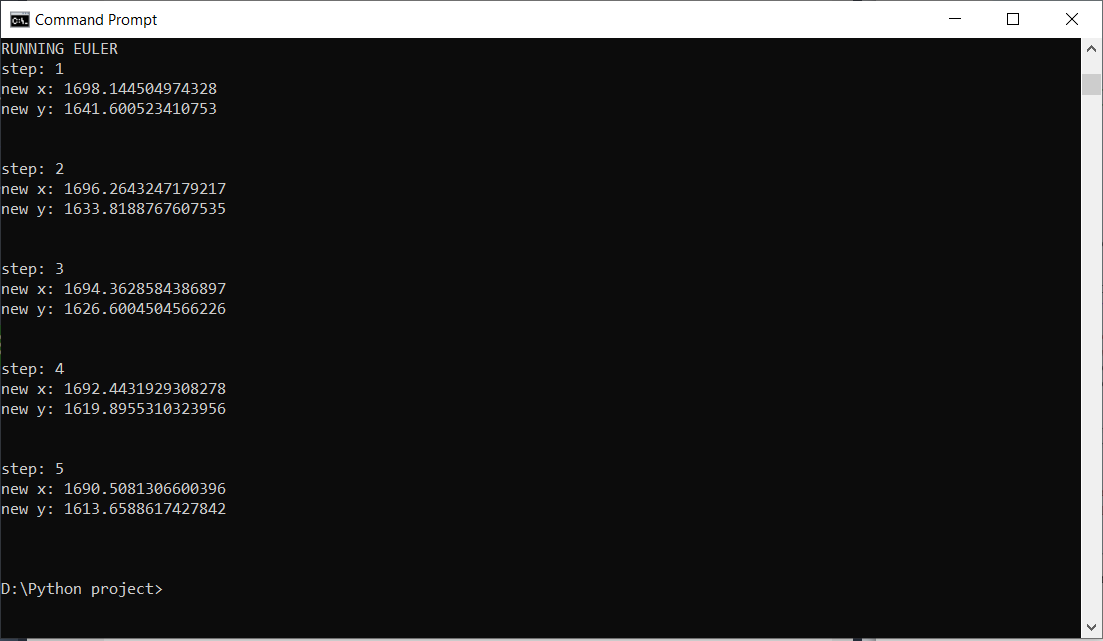
\includegraphics[width=15cm]{Result5_Euler.png}
\end{figure}
\begin{figure}[H]
  \centering
  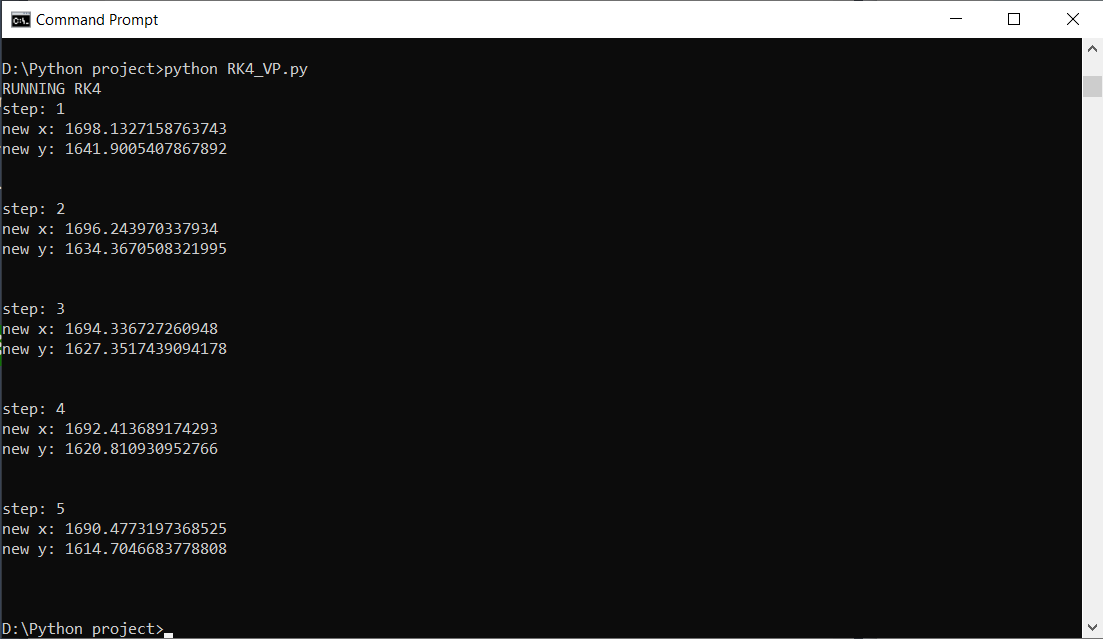
\includegraphics[width=15cm]{Result5_RK4.png}
\end{figure}

The graph below is used to compare to actual data from Van11.

\begin{figure}[H]
  \centering
  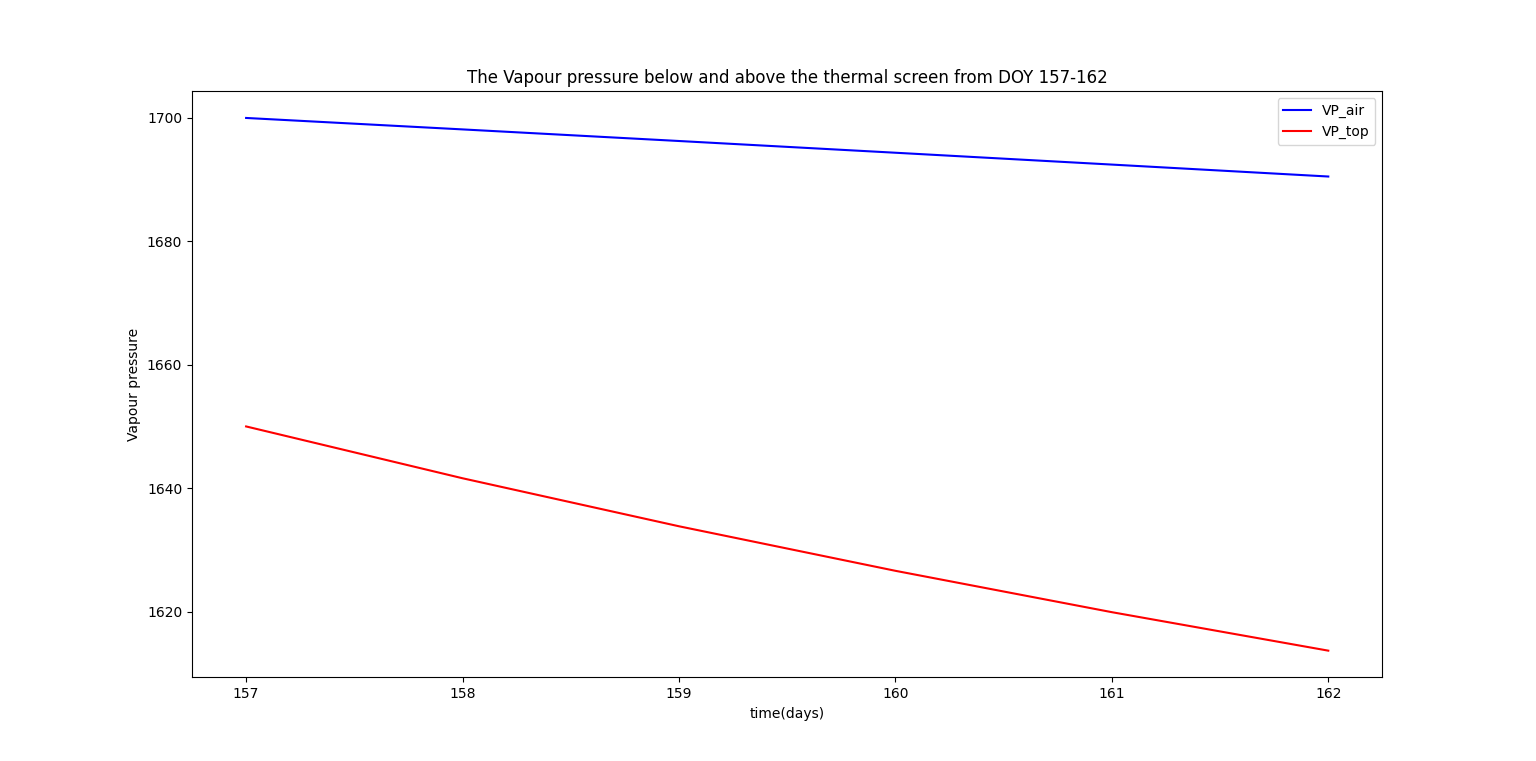
\includegraphics[width=16cm]{VP_compare_Euler.png}
  \caption{Result of Euler method}
\end{figure}
\begin{figure}[H]
  \centering
  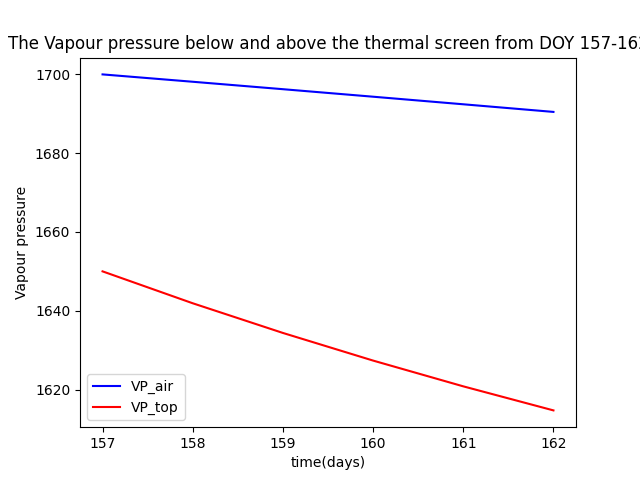
\includegraphics[width=12cm]{VP_compare_RK4.png}
  \caption{Result of RK4 method}
\end{figure}
\begin{figure}[H]
  \centering
  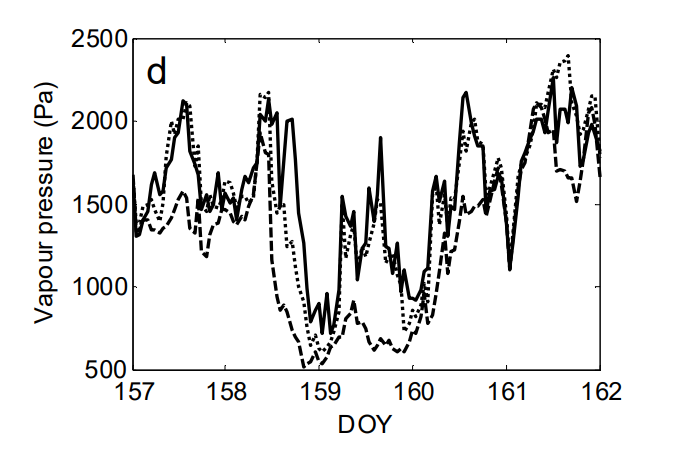
\includegraphics[width=15cm]{VP.png}
  \caption{Actual Data from Van11 page 40}
\end{figure}

Conclusion, even though the predictions indeed resemble the general trends in actual data, they are not close to the actual data as the difference is fairly large and is clearly noticeable in the graph.This can stem from the fact that we lack data and our model is chosen arbitrarily(arbitrary components, the climate of Texas in the data set, and the photosynthetic rate of tomatoes) despite the unawareness of the actual greenhouse model used. So,our model is not cut out for simulating the change in vapour pressure compared to the given model.

\newpage
\printbibliography[heading=bibintoc]

\end{document}

